\documentclass[11pt, a4paper]{article}
\usepackage[utf8]{inputenc}
\usepackage{amsmath,setspace,geometry}
\usepackage{amsthm}
\usepackage{amsfonts}
\usepackage{mathtools}
\mathtoolsset{showonlyrefs}
\usepackage[shortlabels]{enumitem}
\usepackage{rotating}
\usepackage{pdflscape}
\usepackage{graphicx}
\usepackage{bbm}
\usepackage[dvipsnames]{xcolor}
\usepackage[colorlinks=true, linkcolor= RawSienna, citecolor = RawSienna, filecolor = RawSienna, urlcolor = RawSienna, hypertexnames = true, backref = page]{hyperref}
\usepackage[]{natbib} 
\bibpunct[:]{(}{)}{,}{a}{}{,}
\geometry{left = 1.0in,right = 1.0in,top = 1.0in,bottom = 1.0in}
\usepackage[english]{babel}
\usepackage{float}
\usepackage{caption}
\usepackage{subcaption}
\usepackage{tikz}
\usepackage{booktabs}
\usepackage{pdfpages}
\usepackage{threeparttable}
\usepackage{framed}
\usepackage{comment}
\usepackage{lscape}
\usepackage{bm}
\setstretch{1.4}
%\usepackage[tablesfirst,nolists]{endfloat}

\usepackage[T1]{fontenc}
\usepackage{mlmodern}  % 太いComputer Modern
% MLmodernのバグを修正: cf. https://tex.stackexchange.com/questions/646333/size-of-integral-symbol-in-section-header-with-mlmodern
\DeclareFontFamily{OMX}{mlmex}{}
\DeclareFontShape{OMX}{mlmex}{m}{n}{<->mlmex10}{} 
\usepackage{tgtermes} % 数式以外の欧文をTXフォントで上書き

% Theorem numbering setup
\newtheorem{theorem}{Theorem}
\newtheorem{assumption}{Assumption}
\newtheorem{lemma}{Lemma}
\newtheorem{definition}{Definition}
\newtheorem{proposition}{Proposition}
\newtheorem{claim}{Claim}
\newtheorem{corollary}{Corollary}
\newtheorem{example}{Example}
\DeclareMathOperator{\rank}{rank}

\theoremstyle{remark}
\newtheorem{remark}{Remark}

\hyphenation{non-iden-ti-fi-ca-tion}

% Appendix theorem numbering
\makeatletter
\newcommand{\appendixsection}{%
  \setcounter{section}{0}%
  \renewcommand{\thesection}{\Alph{section}}%
  \renewcommand{\thetheorem}{\Alph{section}.\arabic{theorem}}%
  \renewcommand{\thelemma}{\Alph{section}.\arabic{lemma}}%
  \renewcommand{\theproposition}{\Alph{section}.\arabic{proposition}}%
  \renewcommand{\thecorollary}{\Alph{section}.\arabic{corollary}}%
  \renewcommand{\thedefinition}{\Alph{section}.\arabic{definition}}%
}
\makeatother




\title{Revisiting the Identification of the Conduct Parameter in Homogeneous Goods Markets}
\author{Yuri Matsumura\thanks{Department of Economics, Rice University. Email: \href{mailto:yuri.matsumura23@gmail.com}{yuri.matsumura23@gmail.com}} \and Suguru Otani \thanks{Market Design Center, Department of Economics, University of Tokyo. Email: \href{mailto:suguru.otani@e.u-tokyo.ac.jp}{suguru.otani@e.u-tokyo.ac.jp}
}}

\begin{document}

\maketitle
\begin{abstract}
    We revisit the identification of the conduct parameter in homogeneous goods markets.
    \citet{lau1982identifying} shows that the conduct parameter cannot be identified if and only if the demand function is separable but not a specific functional form.
    However, we provide a novel characterization of non-identification and show that the statement in Lau is incorrect.
    Based on our characterization, we provide a new necessary and sufficient condition for the non-identification of the conduct parameter.
    This result implies that the class of inverse demand functions that lead to identification is much broader than Lau considers.
    Our result also emphasizes the insight of \citet{bresnahan1982oligopoly}; the demand rotation instrument is crucial for the identification of the conduct parameter even in more general settings.
\end{abstract}

\noindent\textbf{Keywords:} Identification, Conduct Parameter, Homogenous Goods Market
\vspace{0in}
\newline
\noindent\textbf{JEL Codes:} C5, C13, L1

\bigskip




\newpage
\section{Introduction}
Measuring market power is an important task in the several fields of economics, especially in industrial organization.
While there are several measure of market power, the rise of markup has been a hot topic in both macroeconomics and industrial organization.
(See \citet{millerIndustrial2025} for the detailed survey).
However, when estimating markup, most papers put the restriction on how firms compete, that is, firm conduct.\footnote{
\citet{deloeckerRise2020} uses accounting data and estimate markup based on the production function approach under the assumption of imperfect competition in an output market and perfect competition in input markets.
\citet{dopperRising} uses Nielsen data and estimate markup under the assumption of Bertrand-competition.}
Therefore, while the trend in markup is correctly captured even under the possibility of model misspecification, the magnitude of the rise in markup could be biased.

In the literature on industrial organization, to measure markup under a flexible competition model, the conduct parameter approach has been used.
In this approach, the researcher consider a generalized marginal revenue function with a conduct parameter. 
The equilibrium quantity is determined by the intersection of the marginal revenue function and the marginal cost function.
The conduct parameter approach has been used to measure competitiveness under a flexible competition model: \citet{porterStudy1983}, \citet{genesove1998testing} and \citet{okazaki2022excess}.
In addition to investigating competitiveness, recently the conduct parameter approach has received attention in the literature on the pass-through since \citet{weylPassThrough2013} provides a new insight between the conduct parameter and the pass-through, and some empirical studies estimate the conduct parameter as an intermediate object to investigate the pass-through \citep{millerPassthrough2017}.

A central question in this approach is the identification of the conduct parameter.
As for the identification in homogeneous goods markets, there are two influential papers.
First, \citet{bresnahan1982oligopoly} considers the identification of conduct parameter and marginal cost function in linear demand and linear marginal cost model.
It finds that when the inverse demand function includes a demand shifter, called demand rotation instrument, which changes the slope and intercept of the inverse demand function, the conduct parameter and the parameters of the marginal cost function can be identified.\footnote{Recently, \citet{matsumura2023resolving} provide a detailed condition for the identification.}
Second, \citet{lau1982identifying} considers a more general setting and investigates the conditions under which the conduct parameter is not identified.
It shows that the conduct parameter is not identified if and only if the demand function is separable, except a specific functional form.
In other words, non-separable demand function leads to the identification.
As the inverse demand function with a demand rotation instrument is not separable, this result is regarded as an extension of Bresnahan's idea in a more general setting.


The contribution of this paper is twofold.
First, we point out that the result of Lau is incorrect.
Lau's result implies that when the demand shifter is a scalar, the conduct parameter is never identified except the specific functional form.
This implies that even when an inverse demand function includes a demand rotation instrument, just because the dimension of the demand shifter is one, the conduct parameter is not identified.
The idea of Lau's proof is the following: let $\mathcal{E} = (\theta, MC)$ be the pair of the conduct parameter and the marginal cost function.
Non-identification implies that there is a transformation from the first-order condition under $\mathcal{E}$ to the first-order condition under $\mathcal{E}^{*}$.
Then, an equilibrium quantity satisfies both first-order conditions, which implies that observational equivalence holds.
However, Lau's transformation does not work properly because to keep observational equivalence after the change in a demand rotation instrument, the transformation from $\mathcal{E}$ to $\mathcal{E}^{*}$ requires that marginal cost function in $\mathcal{E}^{*}$ depends on the demand shifter, which violates the exclusive demand shifters assumption.

Second, to resolve the problem, we provide a novel characterization of non-identification and construct a new transformation of the first-order conditions between $\mathcal{E}$ and $\mathcal{E}^{*}$.
While Lau's transformation is constructed by using the derivative of marginal cost with respect to cost shifter, our transformation also uses the derivatives of marginal cost with respect to quantity.
Still, our transformation potentially depends on the demand shifter, and hence to make the transformation valid, we restrict the functional form of the inverse demand function so that the transformation is independent of the demand shifter.
Surprisingly, the resulting class of inverse demand functions shows that non-identification implies that the inverse demand function is separable but also does not have any demand rotation instrument.
In other words, the demand rotation instrument is the key in the identification, which emphasizes that the idea in \citet{bresnahan1982oligopoly} is crucial for the identification of the conduct parameter even in more general settings. 
Additionally, we show that the class of inverse demand functions also works as a sufficient condition for non-identification.
Therefore, the class of inverse demand functions that lead to identification is much broader than Lau considers.



The rest of the paper is organized as follows.
Section \ref{sec:setting} describes the setting.
Section \ref{sec:lau_result} revisits Lau's result and points out the problems in the proof.
Section \ref{sec:nonidentification_characterization} provides a new characterization of non-identification and shows the necessary and sufficient condition for non-identification.
Appendix includes the omitted proofs in the main text and a summary of \citet{goldmanNote1964}.


%In differential product market, \citet{nevoIdentificationOligopolySolution1998} points out the difficulty of identifying the conduct parameter and suggests that testing firm conduct is a better approach in this setting.
%Recently, based on the testable condition from \citet{berry2014identification}, \citet{duarteTesting2024} proposes a test for firm conduct. 
%\citet{magnolfi2022comparison} compare the performance of testing and estimation of the conduct parameter in differential product setting.
%Testing is robust to model misspecification and requires less restrictive instrument variable as long as the menu of models for testing includes the true model.
%Nevertheless, there could be a case where estimating the conduct parameter is better than testing.

%If researchers are interested in the evolution of markup, estimating the conduct parameter is better than testing as testing is more appropriate to see whether the competition is based on price or quantity.



%Based on the critique of \citet{corts1999conduct}, the estimated conduct parameter and the conduct parameter as the elasticity adjusted Lerner index can be different, and hence the consistency of the estimated conduct parameter is questionable.
%However, as \citet{magnolfi2022comparison} also mentions, as long as we assume that the observed data generated from a static competition model with a conduct parameter, the consistency of the estimated conduct parameter can be guaranteed.












\section{Setting}\label{sec:setting}

\subsection{Model and Assumptions}

Consider a homogeneous product market with the aggregate inverse demand and aggregate marginal cost function as $P(Q, X^{d})$ and $MC(Q, X^{s})$ where $X^{d}$ and $X^{s}$ are the vector of exogenous variables.
Let $K_d$ and $K_s$ be the dimension of $X^{d}$ and $X^{s}$, respectively.
We call $X^{d}$ demand shifters and $X^{s}$ cost shifters, and assume the following:
\begin{assumption}\label{assumption:exclusive_shifters}
    The demand shifter $X^{d}$ and the cost shifter $X^{s}$ are exclusive; that is, there is no common variable in $X^{d}$ and $X^{s}$, and $X^{d}$ affects the demand function but not the marginal cost function, and $X^{s}$ affects the marginal cost function but not the demand function; for all $i = 1, \ldots, K_d$ and $j = 1, \ldots, K_s$,
    \begin{align}
        \frac{\partial P}{\partial X^{d}_{i}}(Q, X^{d}) \ne 0, \quad \frac{\partial MC}{\partial X^{s}_{j}}(Q, X^{s}) \ne 0, \quad \frac{\partial P}{\partial X^{s}_{j}}(Q, X^{d}) = 0, \quad \text{and} \quad \frac{\partial MC}{\partial X^{d}_{i}}(Q, X^{s}) = 0.
    \end{align}
\end{assumption}
We can also include some common variables in $X^{d}$ and $X^{s}$, but in that case, we must have at least one exclusive demand shifter and one exclusive cost shifter.
Lau also imposes the following restriction on the inverse demand and the marginal cost function:
\begin{assumption}\label{assumption:twice_differentiable}
    The inverse demand and the marginal cost function are twice continuously differentiable.
\end{assumption}

The equilibrium quantity $Q^e$ is defined as the solution to the following equation:
\begin{align}
    P(Q^e, X^{d}) + \theta Q^e\frac{\partial P}{\partial Q}(Q^e, X^{d}) - MC(Q^e, X^{s}) = 0, \label{eq:foc}
\end{align}
where $\theta$ is called the conduct parameter.
Depending on the value of $\theta$, the relation can nest the equilibrium condition of several models, such as perfect competition ($\theta=0$) and Cournot competition ($\theta=1/N$).

Another interpretation of conduct parameter is obtained by rewriting the equilibrium condition \eqref{eq:foc} as
\begin{align}
    \theta = \frac{P - MC}{P}\varepsilon^{d},
\end{align}
where $\varepsilon^{d}$ is the elasticity of the inverse demand function.
Therefore, the conduct parameter is regarded as an elasticity-adjusted Lerner index.
Recently, \citet{weylPassThrough2013} demonstrate that the pass-through under vast range of imperfect competition models is characterized by the conduct parameter.

\begin{remark}
    \citet{corts1999conduct} criticizes that when the data generation process are outside of the model characterized by \eqref{eq:foc}, the conduct parameter approach cannot consistently estimate the elasticity-adjusted Lerner index. Here, we assume that the data generation process is within the static model characterized by \eqref{eq:foc}. \qed
\end{remark}


Lau does not impose any further restrictions on the inverse demand and the marginal cost function, but it is natural to assume that the equilibrium quantity exists, which needs the following additional assumption:
\begin{assumption}\label{assumption:unique_equilibrium}
    Given an inverse demand function, a conduct parameter, and a marginal cost function, and given $X^{d}$ and $X^{s}$, the derivative of the equilibrium condition with respect to $Q$ is not zero \footnote{By Assumption \ref{assumption:twice_differentiable}, the derivative of the equilibrium condition with respect to $Q$ is finite.}, that is,
    \begin{align}
        (1+\theta)\frac{\partial P}{\partial Q}(Q, X^{d}) + \theta Q\frac{\partial^2 P}{\partial Q^2}(Q, X^{d}) - \frac{\partial MC}{\partial Q}(Q, X^{s}) & \ne 0.
    \end{align}
\end{assumption}



%Based on the exogenous variables, the researcher can identify the reduced form of the equilibrium quantity $Q^e = h_q(X^{d}, X^{s})$.
%Given the inverse demand function, the reduced form of the equilibrium price is $P$, defined as $h_p(X^{d}, X^{s})$, is also identified.
%We put this fact as an assumption:
%\begin{assumption}\label{assumption:reduced_form_identification}
%    The reduced form of the equilibrium quantity $Q^e = h_q(X^{d}, X^{s})$ and the reduced form of the equilibrium price $P^e = h_p(X^{d}, X^{s})$ are identified from the data on price, quantity, and other exogenous variables.
%\end{assumption}


\subsection{Non-identification of the Conduct Parameter and the Marginal Cost}\label{sec:definition_identification}
Suppose that the researcher observes the aggregate price $P$ and the aggregate quantity $Q$, and the vector of exogenous variables $X^{d}$ and $X^{s}$.
Given the inverse demand function, we are interested in the identification of the conduct parameter and the marginal cost function.
While the interest is the identification, we take an indirect approach and specify the conditions under which the model is not identified.
The definition of non-identification is as follows:
\begin{definition}\label{definition:non_identification}
    The conduct parameter and the marginal cost function are not identified if and only if 
    there are two distinct pairs of conduct parameter and marginal cost function, denoted as $(\theta, MC)$ and $(\theta^{*}, MC^{*})$, and for any $X^{d}$ and $X^{s}$, there exist an equilibrium quantity $Q^e$ that satisfies both
    \begin{align}
    P(Q^e, X^{d}) + \theta Q^e\frac{\partial P}{\partial Q}(Q^e, X^{d}) & = MC(Q^e, X^{s}) ,  \label{eq:foc_theta}\\
    P(Q^e, X^{d}) + \theta^{*} Q^e\frac{\partial P}{\partial Q}(Q^e, X^{d}) & = MC^{*}(Q^e, X^{s}).\label{eq:foc_theta_star}
    \end{align}
    The equilibrium quantity $Q^e$ has a reduced form functions $h_q(X^{d}, X^{s})$ and $h_q^{*}(X^{d}, X^{s})$ defined by \eqref{eq:foc_theta} and \eqref{eq:foc_theta_star} respectively are identical.
\end{definition}
In other words, non-identification asks whether given an inverse demand function, it is possible to find two distinct pairs of a conduct parameter and a marginal cost function that lead to observational equivalent equilibrium.
By taking the contraposition of Definition \ref{definition:non_identification}, we can also define the identification of the conduct parameter and marginal cost function:
\begin{definition}\label{definition:identification}
    Identification implies that for any two distinct pairs of conduct parameter and any marginal cost function, there exists a pair of demand shifter $X^{d}$ and $X^{s}$ where the equilibrium quantity $Q^e$ is different, that is, $h_q(X^{d}, X^{s}) \ne h_q^{*}(X^{d}, X^{s})$.
\end{definition}
The intuition is that identification means that any different pairs of conduct parameters and marginal cost functions cannot lead to the same equilibrium quantity under some demand shifter and cost shifter, that is, violates the observational equivalence of the equilibrium quantity.





\section{Lau's Result}\label{sec:lau_result} \label{sec:lau_result}
Based on the above setting, Lau finds that the separability of the inverse demand function and non-identification are equivalent.
\begin{theorem}\label{theorem_lau}
    Given Assumption \ref{assumption:exclusive_shifters}, \ref{assumption:twice_differentiable}, and \ref{assumption:unique_equilibrium},
    the conduct parameter $\theta$ cannot be identified from data on price, quantity, and other exogenous variables alone if and only if the industry inverse demand function is separable in the demand shifter, that is,
    \begin{align}
        P(Q, h(X^{d})), \label{eq:separable_demand}
    \end{align}
    but not take the form, 
    \begin{align}
        P(Q, h(X^{d})) = Q^{-\frac{1}{\theta}}h(X^{d}) + k(Q). \label{eq:identification_separable_demand_lau}
    \end{align}
\end{theorem}
The result says that the shape of the inverse demand function and the dimension of the demand shifter are important for the identification.
First, when the inverse demand function is separable in the demand shifter\footnote{The inverse demand function satisfying \eqref{eq:separable_demand} has weak separability defined in \citet{goldmanNote1964}. See Definition \ref{def:weal_separable} in Appendix \ref{appendix:summary_goldman_uzawa}.}, the conduct parameter is not identified.
For example, \citet{bresnahan1982oligopoly} considers a linear inverse demand function such that
\begin{align}
    P(Q, X^{d}) = \alpha_0 - \alpha_1Q + \alpha_2X^{d}_1 + \alpha_3QX^{d}_1 + \alpha_4X^{d}_2, \label{eq:demand_bresnahan}
\end{align}
where $X^{d}_1$ is called a demand rotation instrument because it can change the slope and intercept of the inverse demand function without changing the equilibrium quantity.
This inverse demand function is not separable in $X^{d}$.
Therefore, under the model with the linear demand and a linear marginal cost, the conduct parameter is identified.

Second, when the demand shifter is a scalar, the inverse demand function \eqref{eq:separable_demand} corresponds to any inverse demand with a scalar demand shifter by putting $h(X^{d})= X^{d}$.
Thus, the conduct parameter can be identified only under the inverse demand function takes the form \eqref{eq:identification_separable_demand_lau} when the demand shifter is a scalar.


\subsection{Discussion}
We now discuss the result of Lau in more detail and point out the problems in the proof.
To see the problem, consider the following inverse demand function:
\begin{align}
    P(Q, X^{d}) = \alpha_0 - \alpha_1Q + \alpha_2X^{d}_1 + \alpha_3QX^{d}_1. \label{eq:demand_counterexample}
\end{align}
We exclude $X^{d}_2$ from \eqref{eq:demand_counterexample}, but it is still non-separable.
Theorem \ref{theorem_lau} implies that the conduct parameter is not identified under this demand because the demand shifter is a scalar.
Note that the difference between \eqref{eq:demand_bresnahan} and \eqref{eq:demand_counterexample} is that the intercept of the inverse demand function changes when $X^{d}_2$ varies.
$X^{d}_1$ still works as a demand rotation instrument, and hence the role of $X^{d}_2$ is almost negligible. 
Unfortunately, it is not clear why adding $X^{d}_2$ to change the intercept is essential for the identification.


Let's revisit why demand rotation works to identify the conduct parameter.
Suppose that the inverse demand function is given by \eqref{eq:demand_counterexample} and that the true conduct is the perfect competition, that is, $\theta = 0$ and the alternative conduct is the monopoly, that is, $\theta^{*} = 1$.
The true and alternative marginal cost functions are also given as linear functions.
Figure \ref{fig:identification_example} illustrates this environment.
Note that the equilibrium quantity is determined by the intersection of the inverse demand function and the marginal cost $MC$ under perfect competition.
The equilibrium quantity under the monopoly is determined by the intersection of the marginal revenue $MR^{*}$ and the marginal cost function $MC^{*}$.

\begin{figure}[p!]
    \begin{center}
        \begin{subfigure}[b]{0.45\textwidth}
            \centering
            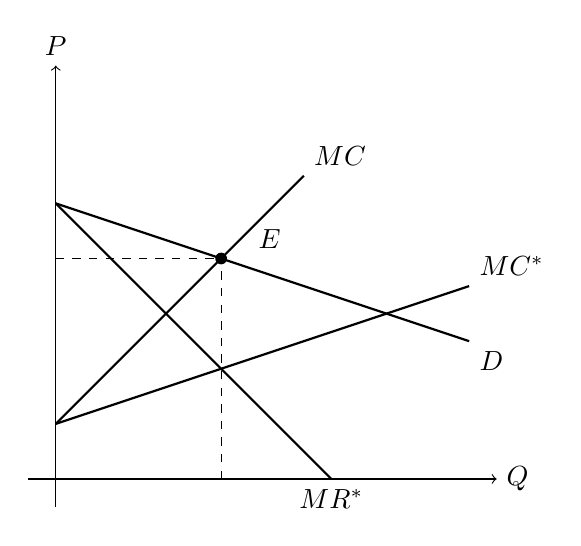
\begin{tikzpicture}[scale = 0.7]
                % Axes
                \draw[->] (-0.5,0) -- (8,0) node[right] {$Q$}; % Horizontal axis
                \draw[->] (0,-0.5) -- (0,7.5) node[above] {$P$}; % Vertical axis

                % Demand Curve (D_1) - passes through (0,5), (3,4), and (7.5,2.5)
                \draw[thick] (0,5) -- (7.5,2.5) node[below right] {$D$};
                % Marginal Revenue (MR_1) - passes through (0,5), (3,2), and (5,0)
                \draw[thick] (0,5) -- (5,0) node[below] {$MR^{*}$};

                % Supply Curve under competition (S^c) - passes through (0,1), (3,4), and (4.5,5.5)
                \draw[thick] (0,1) -- (4.5,5.5) node[above right] {$MC$};

                % Supply Curve under monopoly (S^m) - passes through (0,1), (3,2), and (7.5,3.5)
                \draw[thick] (0,1) -- (7.5,3.5) node[above right] {$MC^{*}$};

                % Equilibrium point (E_1) - intersection of D_1 and S^c at (3,4)
                \node[circle, fill, inner sep=1.5pt] (E1) at (3,4) {};
                \node[above right] at (E1) {$\quad E$};
                \draw[dashed] (3,0) -- (3,4);
                \draw[dashed] (0,4) -- (3,4);
            \end{tikzpicture}
            \caption{Step 1: Observable equivalence holds.}
            \label{fig:identification_example_step_1}
        \end{subfigure}
        \hfill
        \begin{subfigure}[b]{0.45\textwidth}
            \centering
            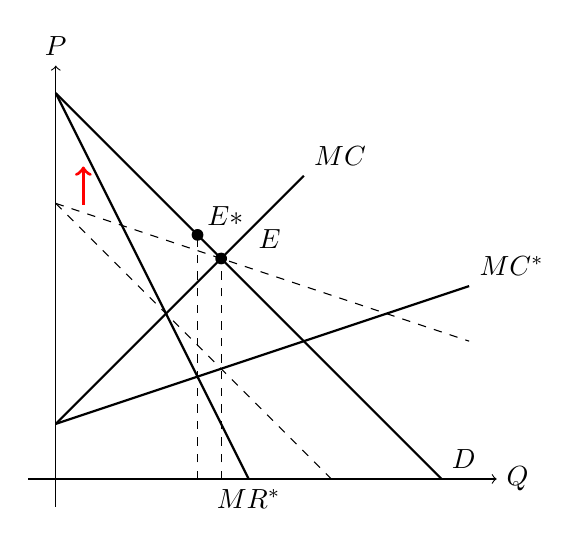
\begin{tikzpicture}[scale = 0.7]
                % Axes
                \draw[->] (-0.5,0) -- (8,0) node[right] {$Q$}; % Horizontal axis
                \draw[->] (0,-0.5) -- (0,7.5) node[above] {$P$}; % Vertical axis

                % Demand Curve (D_1) - passes through (0,5), (3,4), and (7.5,2.5)
                \draw[dashed] (0,5) -- (7.5,2.5) ;
                % Marginal Revenue (MR_1) - passes through (0,5), (3,2), and (5,0)
                \draw[dashed] (0,5) -- (5,0);


                % Shifted Demand Curve (D_1 shifted)
                \draw[thick] (0,7) -- (7,0) node[above right] {$D$};
                % Shifted MR (MR_1 shifted)
                \draw[thick] (0,7) -- (3.5,0) node[below] {$MR^{*}$};

                \draw[-<, very thick, red] (0.5,5) to[out=270,in=90] (0.5,5.5);


                % Supply Curve under competition (S^c) - passes through (0,1), (3,4), and (4.5,5.5)
                \draw[thick] (0,1) -- (4.5,5.5) node[above right] {$MC$};

                % Supply Curve under monopoly (S^m) - passes through (0,1), (3,2), and (7.5,3.5)
                \draw[thick] (0,1) -- (7.5,3.5) node[above right] {$MC^{*}$};

                % Equilibrium point (E_1) - intersection of D_1 and S^c at (3,4)
                \node[circle, fill, inner sep=1.5pt] (E1) at (3,4) {};
                \node[above right] at (E1) {$\quad E$};
                \draw[dashed] (3,0) -- (3,4);

                % Equilibrium point (E_2) - intersection of D_1 and S^c at (7/2,9/2)
                \node[circle, fill, inner sep=1.5pt] (E2) at (18/7,7 - 18/7) {};
                \node[above right] at (E2) {$E{*}$};
                \draw[dashed] (18/7,0) -- (18/7,7 - 18/7);
            \end{tikzpicture}
            \caption{Step 2: Demand rotation changes $D$ and $MR^{*}$}
            \label{fig:identification_example_step_2}
        \end{subfigure}
        \begin{subfigure}[b]{0.45\textwidth}
            \centering
            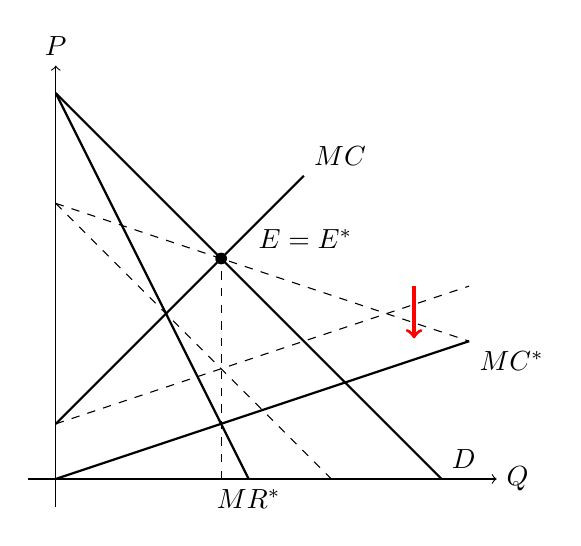
\begin{tikzpicture}[scale = 0.7]
                % Axes
                \draw[->] (-0.5,0) -- (8,0) node[right] {$Q$}; % Horizontal axis
                \draw[->] (0,-0.5) -- (0,7.5) node[above] {$P$}; % Vertical axis

                % Demand Curve (D_1) - passes through (0,5), (3,4), and (7.5,2.5)
                \draw[dashed] (0,5) -- (7.5,2.5) ;
                % Marginal Revenue (MR_1) - passes through (0,5), (3,2), and (5,0)
                \draw[dashed] (0,5) -- (5,0);

                % Shifted Demand Curve (D_1 shifted)
                \draw[thick] (0,7) -- (7,0) node[above right] {$D$};
                % Shifted MR (MR_1 shifted)
                \draw[thick] (0,7) -- (3.5,0) node[below] {$MR^{*}$};

                % Supply Curve under competition (S^c) - passes through (0,1), (3,4), and (4.5,5.5)
                \draw[thick] (0,1) -- (4.5,5.5) node[above right] {$MC$};

                % Supply Curve under monopoly (S^m) - passes through (0,1), (3,2), and (7.5,3.5)
                \draw[dashed] (0,1) -- (7.5,3.5);
                \draw[->, very thick, red] (6.5,3.5) -- (6.5,2.55);

                % Supply Curve under monopoly (S^m) - passes through (0,1), (3,2), and (7.5,3.5)
                \draw[thick] (0,0.0) -- (7.5,2.5) node[below right] {$MC^{*}$};

                % Equilibrium point (E_1) - intersection of D_1 and S^c at (3,4)
                \node[circle, fill, inner sep=1.5pt] (E1) at (3,4) {};
                \node[above right] at (E1) {$\quad E = E^{*}$};
                \draw[dashed] (3,0) -- (3,4);
            \end{tikzpicture}
            \caption{Step 3.1: The intercept of $MC^{*}$ changes along with the demand rotation to keep $E = E^{*}$.}
            \label{fig:identification_example_step_3_1}
        \end{subfigure}
        \hfill
        \begin{subfigure}[b]{0.45\textwidth}
            \centering
            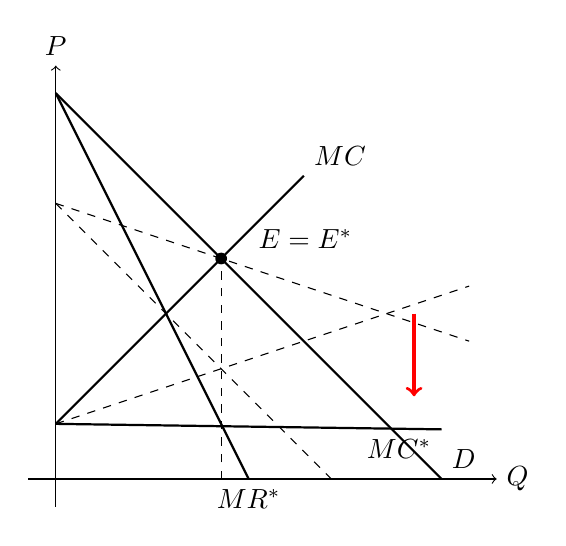
\begin{tikzpicture}[scale = 0.7]
                % Axes
                \draw[->] (-0.5,0) -- (8,0) node[right] {$Q$}; % Horizontal axis
                \draw[->] (0,-0.5) -- (0,7.5) node[above] {$P$}; % Vertical axis

                % Demand Curve (D_1) - passes through (0,5), (3,4), and (7.5,2.5)
                \draw[dashed] (0,5) -- (7.5,2.5) ;
                % Marginal Revenue (MR_1) - passes through (0,5), (3,2), and (5,0)
                \draw[dashed] (0,5) -- (5,0);

                % Shifted Demand Curve (D_1 shifted)
                \draw[thick] (0,7) -- (7,0) node[above right] {$D$};
                % Shifted MR (MR_1 shifted)
                \draw[thick] (0,7) -- (3.5,0) node[below] {$MR^{*}$};

                % Supply Curve under competition (S^c) - passes through (0,1), (3,4), and (4.5,5.5)
                \draw[thick] (0,1) -- (4.5,5.5) node[above right] {$MC$};

                % Supply Curve under monopoly (S^m) - passes through (0,1), (3,2), and (7.5,3.5)
                \draw[dashed] (0,1) -- (7.5,3.5);
                \draw[->, very thick, red] (6.5,3) -- (6.5,1.5);

                % Supply Curve under monopoly (S^m) - passes through (0,1), (3,2), and (7.5,3.5)
                \draw[thick] (0,1) -- (7,0.9) node[below left] {$MC^{*}$};

                % Equilibrium point (E_1) - intersection of D_1 and S^c at (3,4)
                \node[circle, fill, inner sep=1.5pt] (E1) at (3,4) {};
                \node[above right] at (E1) {$\quad E = E^{*}$};
                \draw[dashed] (3,0) -- (3,4);

            \end{tikzpicture}
            \caption{Step 3.2: The slope of $MC^{*}$ changes along with the demand rotation to keep $E = E^{*}$.}
            \label{fig:identification_example_step_3_2}
        \end{subfigure}
    \end{center}
    \caption{Intuition of the role of demand rotation instrument and identification}
    \label{fig:identification_example}
    \vspace{2mm}
    \footnotesize
    Note: The figures illustrate the intuition of how the demand rotation instrument works to identify the conduct parameter.
    $MC$ is the true marginal cost function, and $MC^{*}$ is the marginal cost function that rationalizes the monopoly conduct.
    Step 1 illustrates monopoly and perfect competition are observationally equivalent.
    In step 2, the demand rotation changes the intercept and slope of the demand function without changing the equilibrium point under perfect competition, but changes the equilibrium point under monopoly.
    Step 3 illustrates that to keep the equilibrium point under monopoly, $MC^{*}$ should change along with the demand rotation, which is impossible because the marginal cost function is independent of the demand shifter.
\end{figure}


In Figure \ref{fig:identification_example_step_1}, the perfect competition and the monopoly leads to the same equilibrium $E$.
Then, consider the change in the demand rotation instrument $X^{d}_1$.
In Figure \ref{fig:identification_example_step_2}, the demand rotation changes the intercept and slope of the demand function without changing the equilibrium point under the true model.
Under the monopoly, the new equilibrium point is $E^{*}$, which is different from $E$ and hence the observational equivalence is violated.
So as to lead to the same equilibrium after the change in the demand rotation ($E = E^{*})$, $MC^{*}$ should shift as in Figure \ref{fig:identification_example_step_3_1} and \ref{fig:identification_example_step_3_2}.
Note that we changed only the demand shifter, and hence the cost shifter $X^{s}$ is unchanged.
Thus, for observational equivalence to hold, $MC^{*}$ should also change along with the change in the demand rotation, which implies that $MC^{*}$ is a function of the demand shifter.
However, this is impossible because it violates Assumption \ref{assumption:exclusive_shifters}, that is, the demand shifter should not affect the marginal cost function.
Therefore, even though the demand shifter is a scalar, when it works as a demand rotation instrument, observational equivalence cannot hold for any $X^{d}$ and $X^{s}$, and hence the conduct parameter can be identified.


In Definition \ref{definition:non_identification}, non-identification requires to find two distinct pairs of conduct parameter and marginal cost function that lead to the same equilibrium quantity.
Here, we show only that the demand rotation breaks observational equivalence when the marginal cost is a linear function, hence there is a possibility that observational equivalence can be achieved without depending on the demand shifter under non-linear marginal costs.
However, we will see that the demand rotation instrument can be used to identify the conduct parameter even when the marginal cost is not a linear function.





\section{Characterization of Non-identification}\label{sec:nonidentification_characterization}

Hereafter, we provide an alternative result for the non-identification of the conduct parameter and the marginal cost function. 
The steps are as follows:
First, we derive the necessary condition for non-identification based on Definition \ref{definition:non_identification}.
Then, we provide a transformation between marginal cost functions that leads to observational equivalence under the inverse demand \eqref{eq:demand_counterexample}.
To make the transformation valid, we need to remove the effect of the demand shifter from the transformation, which put restrictions on the inverse demand function.
We then check that under the restricted inverse demand function, we can construct a transformation that leads to observational equivalence, which is the sufficient condition for non-identification.


\subsection{Necessary Condition for Non-identification}

First, we characterizes the non-identification condition based on Definition \ref{definition:non_identification} by following the proof of necessary condition in Lau, but with some modifications.
The characterization is based on the fact that observational equivalence implies that the reduced form of the equilibrium quantity $h_q$ and $h_q^{*}$ are identical for any $X^{d}$ and $X^{s}$.
Therefore, its derivative with respect to the demand and cost shifters, $\nabla h_q$ and $\nabla h_q^{*}$, should be also identical.
Then, by applying the implicit function theorem to the equilibrium condition, we can compute $\nabla h_q$ and $\nabla h_q^{*}$, and hence we can derive the following proposition:
\begin{proposition}\label{proposition:nonidentification_charaterization}
    Non-identification implies that for any $X^{d}$, $X^{s}$, and $Q^e$ under these exogenous variables, we have for $i = 1, \ldots, K_d$,
    \begin{align}
        &\frac{\partial P}{\partial X^{d}_{i}}(Q^e, X^{d}) + \theta^{*} Q^e \frac{\partial^2 P}{\partial X^{d}_{i}\partial Q}(Q^e, X^{d})\\  
        &= \lambda(Q^e, X^{d}, X^{s})\left[ \frac{\partial P}{\partial X^{d}_{i}}(Q^e, X^{d}) + \theta Q^e \frac{\partial^2 P}{\partial X^{d}_{i}\partial Q}(Q^e, X^{d}) \right], \label{eq:nonidentification_demand}
    \end{align}
    and for $j = 1,\ldots, K_s$,
    \begin{align}
        \frac{\partial MC^{*}}{\partial X^{s}_j}(Q^e, X^{s}) = \lambda(Q^e, X^{d}, X^{s}) \frac{\partial MC}{\partial X^{s}_j}(Q^e, X^{s}),\label{eq:nonidentification_marginal_cost}
    \end{align}
    where $\lambda(Q^e, X^{d}, X^{s})$ is defined as
    \begin{align}
        \lambda(Q^e, X^{d}, X^{s}) \equiv \frac{(1+\theta^{*})\frac{\partial P}{\partial Q}(Q^e, X^{d}) + \theta^{*} Q^e\frac{\partial^2 P}{\partial Q^2}(Q^e, X^{d}) - \frac{\partial MC^{*}}{\partial Q}(Q^e, X^{s})}{(1+\theta)\frac{\partial P}{\partial Q}(Q^e, X^{d}) + \theta Q^e\frac{\partial^2 P}{\partial Q^2}(Q^e, X^{d}) - \frac{\partial MC}{\partial Q}(Q^e, X^{s})}. \label{eq:lambda_foc}
    \end{align}
\end{proposition}
See Appendix \ref{appendix:proof} for the detailed proof.
\eqref{eq:nonidentification_demand} and \eqref{eq:nonidentification_marginal_cost} implies that when non-identification holds, the derivative of the marginal revenue with $\theta$ can be transformed into the derivative of the marginal revenue with $\theta^{*}$, and the derivative of the marginal cost $MC$ with respect to $X^{s}$ can be transformed into the derivative of the marginal cost $MC^{*}$ with respect to $X^{s}$ by the same transformation using $\lambda(Q^e, X^{d}, X^{s})$.

These transformations cannot be always valid because the transformed marginal revenue is affected by cost shifter $X^{s}$, and the transformed marginal cost is affected by demand shifter $X^{d}$ through $\lambda(Q^e, X^{d}, X^{s})$.
The transformation is valid for the marginal revenue when we can remove the effect of $X^{s}$ from $\lambda(Q^e, X^{d}, X^{s})$, but in this case $\lambda(Q^e, X^{d}, X^{s})$ depends on $X^{d}$, and hence the transformation is not valid for the marginal cost.

\begin{remark}\label{remark:lau_argument_transformation}
While Lau uses the same logic in Lemma \ref{proposition:nonidentification_charaterization}, he obtains a slightly different equation from \eqref{eq:nonidentification_marginal_cost}.
Equation (15) in Lau is
\begin{align}
    \frac{\partial MC^{*}}{\partial X^{s}_j}(Q, X^{s}) = \lambda'(Q, X^{s}) \frac{\partial MC}{\partial X^{s}_j}(Q, X^{s}),\quad \forall Q, X^{s}, \label{eq:nonidentification_marginal_cost_lau}
\end{align}
where $\lambda'(Q, X^{s})$ depends only on $Q$ and $X^{s}$.
Then he concludes that there is a transformation $T$ such that 
\begin{align}
    MC^{*}(Q, X^{s}) = T(MC(Q, X^{s}), Q). \label{eq:mc_transformation_lau}
\end{align}
The existence of the transformation $T$ is shown by integrating \eqref{eq:nonidentification_marginal_cost_lau} with respect to $X^{s}$ when $X^{s}$ is a scalar, and by applying Lemma \ref{lemma_1_GU} from \citet{goldmanNote1964} when $X^{s}$ is a vector.

In fact, it can be verified that Lau derives \eqref{eq:nonidentification_demand} and \eqref{eq:nonidentification_marginal_cost} in his proof, but ignores $X^{d}$ from $\lambda(Q, X^{d}, X^{s})$ and defines \eqref{eq:nonidentification_marginal_cost_lau}.
As long as $X^{d}$ cannot be removed from $\lambda(Q, X^{d}, X^{s})$, $T$ also depends on $X^{d}$ and hence $T$ cannot be a valid transformation between $MC$ and $MC^{*}$.
Unfortunately, Lau does not argue why $X^{d}$ is removed.
\qed
\end{remark}

To resolve the problem in Lau, we further rewrite \eqref{eq:nonidentification_demand} and \eqref{eq:nonidentification_marginal_cost} so that we can construct a valid transformation based on 
a new characterization of non-identification using both \eqref{eq:nonidentification_demand} and \eqref{eq:nonidentification_marginal_cost}.
First, we rewrite \eqref{eq:nonidentification_demand} based on the derivative of $MC$ and $MC^{*}$ with respect to $Q$ at the equilibrium quantity: for $i = 1, \ldots, K_d$,
\begin{align}
    \frac{\partial MC^{*}}{\partial Q}(Q^e, X^{s}) =D_i(Q^e, X^{d}) + C_i(Q^e, X^{d})\frac{\partial MC}{\partial Q}(Q^e, X^{s}),\label{eq:mc_transformation_quantity}
\end{align}
where $C_i(Q, X^{d})$ and $D_i(Q, X^{d})$ are defined as
\begin{align}
    C_i(Q, X^{d}) \equiv \frac{\frac{\partial P}{\partial X^{d}_i}(Q, X^{d}) + \theta^{*} Q\frac{\partial^2 P}{\partial X^{d}_{i}\partial Q}(Q, X^{d}) }{\frac{\partial P}{\partial X^{d}_i}(Q, X^{d}) + \theta Q\frac{\partial^2 P}{\partial X^{d}_{i}\partial Q}(Q, X^{d}) },\label{eq:ratio_marginal_revenue}
\end{align}
and
\begin{align}
    D_i(Q, X^{d}) & \equiv\frac{(\theta^{*} - \theta)}{\frac{\partial P}{\partial X^{d}_i}(Q, X^{d}) + \theta Q\frac{\partial^2 P}{\partial X^{d}_{i}\partial Q}(Q, X^{d})}\Bigg[\frac{\partial P}{\partial Q}(Q, X^{d}) \frac{\partial P}{\partial X^{d}_i}(Q, X^{d})\\
    &\quad + Q\frac{\partial^2 P}{\partial Q^2}(Q, X^{d}) \frac{\partial P}{\partial X^{d}_i}(Q, X^{d}) - Q \frac{\partial P}{\partial Q}(Q, X^{d}) \frac{\partial^2 P}{\partial X^{d}_i\partial Q}(Q, X^{d}) \Bigg]\label{eq:intercation_derivative_demand}
\end{align}

%This can be more simplified as (we suppress the arguments of the functions for brevity),
%\begin{align}
    %&(1+ \theta^{*})\frac{\partial P}{\partial Q} + \theta^{*} Q\frac{\partial^2 P}{\partial Q^2} - \frac{\frac{\partial P}{\partial X^{d}_i} + \theta^{*} Q\frac{\partial^2 P}{\partial X^{d}_{i}\partial Q} }{\frac{\partial P}{\partial X^{d}_i} + \theta Q\frac{\partial^2 P}{\partial X^{d}_{i}\partial Q} }\left[(1+ \theta) \frac{\partial P}{\partial Q} + \theta Q\frac{\partial^2 P}{\partial Q^2}\right]\\
    %&= \frac{1}{\frac{\partial P}{\partial X^{d}_i} + \theta\frac{\partial^2 P}{\partial X^{d}_{i}\partial Q}Q}\left[\left((1 + \theta^{*}) \frac{\partial P}{\partial Q} + \theta^{*} Q\frac{\partial^2 P}{\partial  Q^2}\right)\left(\frac{\partial P}{\partial X^{d}_i} + \theta Q\frac{\partial^2 P}{\partial X^{d}_{i}\partial Q}\right)\right]\\
    %&\quad - \frac{1}{\frac{\partial P}{\partial X^{d}_i} + \theta\frac{\partial^2 P}{\partial X^{d}_{i}\partial Q}Q}\left[\left( (1 + \theta) \frac{\partial P}{\partial Q} + \theta Q\frac{\partial^2 P}{\partial Q^2}\right)\left(\frac{\partial P}{\partial X^{d}_i} + \theta^{*} Q\frac{\partial^2 P}{\partial X^{d}_{i}\partial Q}\right)\right]\\
    %& = 
%\end{align}



Next, \eqref{eq:nonidentification_demand} and \eqref{eq:nonidentification_marginal_cost} imply that for $i = 1, \ldots, K_d$ and $j = 1, \ldots, K_s$,
\begin{align}
    \lambda(Q^e, X^{d}, X^{s}) =  \frac{\frac{\partial MC^{*}}{\partial X^{s}_j}(Q^e, X^{s})}{\frac{\partial MC}{\partial X^{s}_j}(Q^e, X^{s})} =  \frac{\frac{\partial P}{\partial X^{d}_i}(Q^e, X^{d}) + \theta^{*} Q^e\frac{\partial^2 P}{\partial X^{d}_{i}\partial Q}(Q^e, X^{d}) }{\frac{\partial P}{\partial X^{d}_i}(Q^e, X^{d}) + \theta Q^e\frac{\partial^2 P}{\partial X^{d}_{i}\partial Q}(Q^e, X^{d})},
\end{align}
and from the second equality, we have for $i = 1, \ldots, K_d$ and $j = 1, \ldots, K_s$,
\begin{align}
    \frac{\partial MC^{*}}{\partial X^{s}_j}(Q^e, X^{s}) = C_i(Q^e, X^{d})\frac{\partial MC}{\partial X^{s}_j}(Q^e, X^{s}).\label{eq:mc_transformation_cost_shifter}
\end{align}
Equations \eqref{eq:mc_transformation_quantity} and \eqref{eq:mc_transformation_cost_shifter}  can be interpreted as transformations of the derivatives of the marginal cost functions $MC$ and $MC^{*}$ with respect to $Q$ and $X^{s}$ at the equilibrium quantity.
As we saw in Section \ref{sec:lau_result}, for the transformations to hold universally for any $Q^e$ and $X^{s}$, they must be independent of $X^{d}$.
If the dependence holds, while demand rotation does not change the equilibrium quantity $Q^e$, it additionally changes $MC^{*}$ via $C_i$ and $D_i$.
This is the scenario illustrated in Figure \ref{fig:identification_example}, which violates Assumption \ref{assumption:exclusive_shifters}. 
Therefore, in order for the transformations to be valid, both $C_i$ and $D_i$ must be independent of $X^{d}$.

Because $C_i$ and $D_i$ consist of the inverse demand function, making $C_i$ and $D_i$ independent of $X^{d}$ can restrict the form of the inverse demand function.
For this purpose, we take the derivative of $C_i$ and $D_i$ with respect to $X^{d}$ and set it to zero.
This requires the following assumption:
\begin{assumption}\label{assumption:three_times_differentiable}
    The inverse demand function is three times continuously differentiable.
    The marginal cost function is twice continuously differentiable.
\end{assumption}
This assumption puts a stronger restriction on the inverse demand function than Assumption \ref{assumption:twice_differentiable}.
However, this is necessary for the investigation because $C_i$ and $D_i$ already include second-order derivatives of the inverse demand function, and hence to take a derivative of $C_i$ and $D_i$ with respect to $X^{d}$, we need to assume three-times differentiability.

\begin{remark}
    Another justification for this assumption is that Lau assumes twice-continuously differentiability to apply Lemma \ref{lemma_1_GU} to get the transformation between $MC$ and $MC^{*}$, which does not work as \eqref{eq:nonidentification_marginal_cost_lau} depends on $X^{d}$.
    To make the argument work, it is also required to take a derivative of $\lambda(Q^e, X^{d}, X^{s})$ with respect to $X^{d}$ and set it to zero, which requires three-times differentiability of inverse demand function.
    \qed
\end{remark}


Before we characterize the class of inverse demand functions that make $C_i$ and $D_i$ independent of $X^{d}$, we first check the condition that makes $C_i$ and $D_i$ not well-defined.
This implies that \eqref{eq:ratio_marginal_revenue} and \eqref{eq:intercation_derivative_demand} are violated, and hence the identification holds.
To see when \eqref{eq:ratio_marginal_revenue} and \eqref{eq:intercation_derivative_demand} are violated, it is sufficient to consider the case where the denominator of $C_i$ and $D_i$ is zero: for any $Q$ and $X^{d}$,
\begin{align}
    \frac{\partial P}{\partial X^{d}_i}(Q, X^{d}) + \theta Q\frac{\partial^2 P}{\partial X^{d}_{i}\partial Q}(Q, X^{d}) = 0. \label{eq:identification_condition_separable}
\end{align}
Note that \eqref{eq:identification_condition_separable} can be rewritten as
\begin{align}
    \frac{\partial }{\partial X^{d}_i}\left( P(Q, X^{d}) + \theta Q \frac{\partial P}{\partial Q}(Q, X^{d})\right) = 0,
\end{align}
which is the derivative of the marginal revenue under $\theta$ with respect to $X^{d}_i$.
Thus, \eqref{eq:identification_condition_separable} implies that the marginal revenue under $\theta$ is not affected by $X^{d}_i$.

$C_i$ and $D_i$ consist of the derivative of the inverse demand function, and Assumption \ref{assumption:three_times_differentiable} guarantees that these derivatives are finite.
Therefore, the numerator and the denominator of $C_i$ and $D_i$ cannot take infinite values.
In this case, no matter what value of the numerator of $C_i$ and $D_i$ is, \eqref{eq:ratio_marginal_revenue} and \eqref{eq:intercation_derivative_demand} are violated when the denominator of $C_i$ and $D_i$ is zero, under which $C_i$ and $D_i$ will be infinite or indeterminate.
In fact, \eqref{eq:identification_condition_separable} leads to a class of inverse demand function that always leads to identification.
\begin{lemma}\label{lemma:identification_condition_separable}
    Suppose that $\theta \ne 0$.  
    Let $\mathcal{I}$ be the set of indices of the demand shifters where \eqref{eq:identification_condition_separable} holds.
    Then, the conduct parameter and the marginal cost function are identified when the inverse demand function is such that
    \begin{align}
        P(Q, X^{d}) = Q^{-\frac{1}{\theta}}h(X^{d}) + k(Q, X^{d}_{-\mathcal{I}}), \label{eq:identification_separable_demand}
    \end{align}
    where $X^{d}_{-\mathcal{I}}$ is the vector of demand shifters whose index is not in $\mathcal{I}$, and $h(\cdot)$ and $k(\cdot)$ are twice continuously differentiable functions.
\end{lemma}
See Appendix \ref{appendix:proof} for the proof.
Under \eqref{eq:identification_separable_demand}, the equilibrium condition \eqref{eq:foc_theta} is given as
\begin{align}
    k(Q, X^{d}_{-\mathcal{I}}) + \theta Qk'(Q, X^{d}_{-\mathcal{I}}) = MC(Q, X^{s}),
\end{align}
which implies that the equilibrium quantity is not affected by the change in $X^{d}_i$ for any $i \in \mathcal{I}$.
Therefore, when the conduct parameter is $\theta$ and under \eqref{eq:identification_separable_demand}, all demand shifters whose index is in $\mathcal{I}$ always work as a demand rotation instrument.
On the other hand, for any other conduct parameter $\theta^{*}$, the marginal revenue is always affected by $X^{d}_i$, and hence the equilibrium quantity under the model with $\theta^{*}$ is different from the equilibrium quantity under the model with $\theta$.
Therefore, the observational equivalence is always violated, which implies that the conduct parameter and the marginal cost function are identified.



\begin{remark}
    Lau also considers the case where \eqref{eq:identification_condition_separable} holds, but only the case when the demand shifter is a scalar, that is, $K_d = 1$.
    Then $k(Q, X^{d}_{-\mathcal{I}})$ is reduced to $k(Q)$.
    Thus, \eqref{eq:identification_separable_demand} is reduced to the inverse demand function \eqref{eq:identification_separable_demand_lau} in Theorem \ref{theorem_lau}.
    However, our result is an extension because it considers the case where the demand shifter is a vector. \qed
\end{remark}

Now, suppose that \eqref{eq:identification_condition_separable} does not hold for all demand shifters.
Then, we can characterize the class of inverse demand functions by considering the case where $C_i$ and $D_i$ are independent of $X^{d}$.
The following proposition shows that there is a unique class of inverse demand functions that satisfies this condition:
\begin{proposition}\label{proposition:nonidentification_inverse_demand}
    Suppose that \eqref{eq:identification_condition_separable} does not hold for any $i = 1, \ldots, K_d$.
    Then, $C_i(Q, X^{d})$ and $D_i(Q, X^{d})$ are independent of $X^{d}$ if and only if the inverse demand function is given as \begin{align}
        P(Q, X^{d}) = Q^{\alpha_1}h(X^{d}) + k(Q), \label{eq:nonidentification_inverse_demand}
    \end{align}
    where $\alpha_1 \in \mathbb{R}$ is a constant but not $\alpha_1 = -\frac{1}{\theta}$, and $h(\cdot)$ and $k(\cdot)$ are twice continuously differentiable functions.
\end{proposition}
See Appendix \ref{appendix:proof} for the proof.
As in Theorem \ref{theorem_lau}, non-identification implies separable inverse demand functions.
However, our result tells more about under what type of separable function the non-identification holds.
Observe that when $\alpha_1 \ne 0$, the demand shifter changes only the slope of the inverse demand function, and when $\alpha_1 = 0$, the demand shifter changes only the intercept of the inverse demand function.
Therefore, we cannot have demand rotation instruments under \eqref{eq:nonidentification_inverse_demand}.
This result implies that demand rotation instrument is a key to identify the conduct parameter and the marginal cost function, which emphasizes the idea of \citet{bresnahan1982oligopoly} in more general setting.
Thus, whenever we have a set of demand shifters that can work as demand rotation instrument, the conduct parameter and the marginal cost function are identified.

Additionally, unlike in Theorem \ref{theorem_lau}, our result implies that the dimension of the demand shifter does not matter for the identification because our result holds for any dimension of the demand shifter.
When the inverse demand function is \eqref{eq:demand_counterexample}, $C_i$ and $D_i$ are given as
\begin{align}
    C_i(Q, X^{d}) = \frac{\alpha_2 + \theta\alpha_3Q}{\alpha_2 + \theta^{*}\alpha_3Q},\quad \text{ and }\quad  D_i(Q, X^{d}) =  (\theta^{*} - \theta)(-\alpha_1 + \alpha_3X^{d}).
\end{align}
This implies that the transformation \eqref{eq:mc_transformation_quantity} is not valid because $D_i(Q, X^{d})$ depends on $X^{d}$.
Therefore, any $MC^{*}$ that leads to observational equivalence with $MC$ should depend on the demand shifter, under which non-identification is impossible.
While Figure \ref{fig:identification_example} considers the case where the marginal cost function is linear, \eqref{eq:demand_bresnahan} and \eqref{eq:demand_counterexample} have the same power to identify the conduct parameter and the marginal cost in more general setting because both functions include a demand rotation instrument.



\subsection{Sufficient Condition for Non-identification}
Because we have characterizes the class of inverse demand functions implied by non-identification, we are interested in whether the class of inverse demand functions can lead to non-identification.
To see whether the inverse demand function \eqref{eq:nonidentification_inverse_demand} can lead to non-identification, we need to check whether there exists a transformation $T$ such that
\begin{align}
    P(Q, X^{d}) + \theta^{*} Q \frac{\partial P}{\partial Q}(Q, X^{d}) = T\left(P(Q, X^{d}) + \frac{\partial P}{\partial Q}(Q, X^{d}), Q\right)
\end{align}
and
\begin{align}
    MC(Q, X^{s}) = T\left(MC(Q, X^{s}), Q\right).
\end{align}
This transforms the marginal revenue under $\theta$ to the marginal revenue under $\theta^{*}$ and the marginal cost $MC$ to the marginal cost $MC^{*}$.
Then, when an equilibrium quantity $Q^e$ satisfies the equilibrium condition under $(\theta, MC)$, $Q^e$ also satisfies the equilibrium condition under $(\theta^{*}, MC^{*})$ because by applying the transformation to the equilibrium condition under $(\theta, MC)$, we have that
\begin{align}
    T\left(P(Q^e, X^{d}) + \theta Q^e \frac{\partial P}{\partial Q}(Q^e, X^{d}), Q^e\right)&= T\left(MC(Q^e, X^{s}), Q^e\right)\\
    P(Q^e, X^{d}) + \theta^{*} Q^e \frac{\partial P}{\partial Q}(Q^e, X^{d})&= MC^{*}(Q^e, X^{s}).
\end{align}

In fact, \eqref{eq:mc_transformation_quantity} can give us a sufficient condition for non-identification, which implies that by using the inverse demand function \eqref{eq:nonidentification_inverse_demand}, we can construct the transformation.
We state this result as a proposition and the proof is given in Appendix \ref{appendix:proof}:
\begin{proposition}\label{proposition:sufficient_nonidentification}
    Given the inverse demand function \eqref{eq:nonidentification_inverse_demand} where $\alpha_1 \ne -\frac{1}{\theta}$, there exists a transformation $T$ between the equilibrium conditions under $(\theta, MC)$ and $(\theta^{*}, MC^{*})$.
    Therefore, non-identification of the conduct parameter and the marginal cost function holds under \eqref{eq:nonidentification_inverse_demand}.
\end{proposition}


\begin{remark}
    Lau's sufficiency proof is incomplete because it implicitly assumes that there exists a transformation $T$ under a separable inverse demand function \eqref{eq:separable_demand}.
    Proposition \ref{proposition:sufficient_nonidentification} shows that more specific separable inverse demand function can lead to a transformation that leads to non-identification. \qed
\end{remark}

\section{Identification of the Model}

So far, we have characterized the non-identification problem given an inverse demand function, that is, we have assumed that the inverse demand function is already identified.
In this section, we consider the identification of the entire model.

Before we proceed, we summarize the results in the previous section as a theorem:
\begin{theorem}\label{theorem:identification_characterization}
    Given Assumption \ref{assumption:exclusive_shifters}, \ref{assumption:unique_equilibrium}, and \ref{assumption:three_times_differentiable}, the conduct parameter $\theta$ cannot be identified from data on price, quantity, and other exogenous variables alone if and only if the industry inverse demand function is given as
    \begin{align}
        P(Q, X^{d}) = Q^{\alpha_1}h(X^{d}) + k(Q)
    \end{align}
    where $\alpha_1 \in \mathbb{R}$ is a constant but not $\alpha_1 = -\frac{1}{\theta}$, and $h(\cdot)$ and $k(\cdot)$ are twice continuously differentiable functions.
\end{theorem}

First, we can at least assume that the reduced-form of the equilibrium quantity and the equilibrium price are identified:
\begin{assumption}\label{assumption:reduced_form}
    The reduced-form of the equilibrium quantity and the equilibrium price are identified:
    \begin{align}
        Q^e = h_q(X^{d}, X^{s}), \quad P^e = h_p(X^{d}, X^{s}).
    \end{align}
\end{assumption}
This is due to the variation in the demand and cost shifters.
However, this does not imply that the inverse demand function is identified, and hence we need to consider the identification of the inverse demand function.

Recall that Lemma \ref{lemma:identification_condition_separable} characterizes the class of inverse demand function that always leads to identification of the conduct parameter and the marginal cost function.
Unfortunately, with data generated by a model with the inverse demand function \eqref{eq:identification_separable_demand}, we cannot identify the inverse demand function, and hence the identification of the conduct parameter and the marginal cost function is impossible.
The intuition is that when the true inverse demand function is \eqref{eq:identification_separable_demand}, the equilibrium quantity and the equilibrium price are not affected by the demand shifters that work as a demand rotation instrument.
We state this result as a proposition and the proof is given in Appendix \ref{appendix:proof}:
\begin{proposition}\label{proposition:nonidentification_separable_demand}
    When the data is generated from a model with the inverse demand function \eqref{eq:identification_separable_demand}, the inverse demand function is not identified, and hence the conduct parameter and the marginal cost function are not identified.
\end{proposition}




Now, we consider whether the inverse demand function can be identified when the conduct parameter and the marginal cost function are not identified.
Again, unfortunately, we have the following result:
\begin{proposition}\label{proposition:nonidentification_inverse_demand_with_nonidentifed_conduct_parameter}
    The inverse demand function \eqref{eq:nonidentification_inverse_demand} where $\alpha_1 \ne -\frac{1}{\theta}$ cannot be identified.
\end{proposition}






As the inverse demand function \eqref{eq:nonidentification_inverse_demand} leads to the non-identification of the conduct parameter and the marginal cost function, any other inverse demand function can achieve the identification.
Additionally, non-identification of \eqref{eq:nonidentification_inverse_demand} implies that the inverse demand function that leads to the identification of the conduct parameter and the marginal cost function can be identified from the observed information.

Therefore, we have the following corollary.
\begin{corollary}
    When the inverse demand function does not satisfy \eqref{eq:nonidentification_inverse_demand} for any $\alpha_1 \in \mathbb{R}$, all model components, the inverse demand function, the conduct parameter, and the marginal cost function, are identified.
\end{corollary}








% 言い換えると,non-identificationを満たすような需要関数の場合,demand shifterの変化はinverse demand functionの傾きだけを変化させるし,demand shifterはsingle indexとして集約されている

%疑問としては,nonidentificationが成り立つようなinverse demand functionでなければ,常にinverse demand functionは識別できるのか?
%懸念としては,あるdemand shifterが常にdemand rotation instrumentとして動いてしまうと,inverse demand functionが識別できなくなってしまう
%おそらく,demand shifterの動きが組み合わさってdemand rotationとして動いている場合には個々のdemand shifterの動きにある程度のvariationがあればinverse demand functionは識別できると思われる.
% demand functionがnonidentificationを満たすものであれば,そのinverse demand functionが識別できないことを示せば,対偶として,inverse demand functionが識別できるのであれば,nonidentificationが成立するようなinverse demand functionの形にはならないことを示せる.




\section{Conclusion and Discussion}

This paper revisited the identification of the conduct parameter in homogeneous product market.
In the literature, Lau considers the identification problem in a fairly generalized setting.
While Lau characterizes the non-identification condition, we point out some problems in Lau's paper and provide a novel characterization of the non-identification condition.
Based on the new characterization, we find that the non-identification is equivalent to the absence of demand shifters that works as demand rotation instrument proposed in \citet{bresnahan1982oligopoly}.
We then consider the identification of the all primitives in the model and show that when some demand shifters always work as demand rotation instruments, the inverse demand function cannot be identified, which immediately implies that the conduct parameter and the marginal cost function are also not identified.
Therefore, while demand rotation instrument is a key for the identification of the conduct parameter, it could be prevent us from the identification.



The literature has only consider the identification problem when aggregate data are available.
When firms are symmetric, the firm-level first-order condition can be considered and then it is natural to think that all firms share the same conduct parameter.




\bibliographystyle{aer}
\bibliography{conduct_parameter.bib}


\newpage
\appendix
\appendixsection
\numberwithin{theorem}{section}
\numberwithin{lemma}{section}
\numberwithin{proposition}{section}
\numberwithin{corollary}{section}
\numberwithin{definition}{section}
\numberwithin{example}{section}
\numberwithin{assumption}{section}
\numberwithin{claim}{section}

\begin{center}
\huge\textbf{Appendix}
\end{center}
\vspace{1mm}

\section{Omitted Proofs}\label{appendix:proof}
In this section, we provide the proofs of the lemmas and theorems in the main text.
In what follows, we suppress the arguments of functions when no confusion arises.


\subsection{Proof of Proposition \ref{proposition:nonidentification_charaterization}}
Assume that given $X^{d}$ and $X^{s}$, we can solve the equilibrium condition for the equilibrium quantity $Q^e$.
For notational simplicity, we define
\begin{align}
    F(Q^e, X^{d}, X^{s}; \theta, MC) \equiv P(Q^e, X^{d}) + \theta Q^e\frac{\partial P}{\partial Q}(Q^e, X^{d}) - MC(Q^e, X^{s}).
\end{align}
Then, by Assumption \ref{assumption:unique_equilibrium}, we can apply the implicit function theorem, and for the reduced-form equation $Q^e = h_q(X^{d}, X^{s})$, the gradient of the reduced-form function $h_q$ with respect to $X^{d}$ and $X^{s}$ is given by
\begin{align}
    \nabla h_q(X^{d}, X^{s}) =  \left( -\dfrac{\frac{\partial F}{\partial X^{m}_{i}}(h_q(X^{d}, X^{s}), X^{d}, X^{s})}{\frac{\partial F}{\partial Q}(h_q(X^{d}, X^{s}), X^{d}, X^{s})} \right)_{\substack{m = d, s\\ i = 1, \ldots, K_m}}. \label{eq:foc_derivative_demand_supply}
\end{align}
The derivatives of $F$ for each variable are for $i = 1, \ldots, K_d$ and $i = 1, \ldots, K_s$,
\begin{align}
    \frac{\partial F}{\partial X^{d}_i}(Q^e, X^{d}, X^{s}; \theta, MC) & =  \frac{\partial P}{\partial X^{d}_{i}}(Q^e, X^{d}) + \theta\frac{\partial^2 P}{\partial X^{d}_{i}\partial Q}(Q^e, X^{d})Q^e,\\
    \frac{\partial F}{\partial X^{s}_i}(Q^e, X^{d}, X^{s}; \theta, MC) & =  -\frac{\partial MC}{\partial X^{s}_{i}}(Q^e, X^{s}), \\
    \frac{\partial F}{\partial Q}(Q^e, X^{d}, X^{s}; \theta, MC) & = (1+\theta)\frac{\partial P}{\partial Q}(Q^e, X^{d}) + \theta Q^e\frac{\partial^2 P}{\partial Q^2}(Q^e, X^{d}) - \frac{\partial MC}{\partial Q}(Q^e, X^{s}).
\end{align}
Thus, the derivative of $h$ with respect to $X^{d}_i$ and $X^{s}_i$ are given as for $i = 1, \ldots, K_d$ and $i = 1, \ldots, K_s$,
\begin{align}
    \frac{\partial h_q}{\partial X^{d}_{i}}(X^{d}, X^{s}) = -\frac{\frac{\partial P}{\partial X^{d}_{i}}(Q^e, X^{d}) + \theta Q^e \frac{\partial^2 P}{\partial X^{d}_{i}\partial Q}(Q^e, X^{d}) }{(1+\theta)\frac{\partial P}{\partial Q}(Q^e, X^{d}) + \theta  Q^e\frac{\partial^2 P}{\partial Q^2}(Q^e, X^{d}) - \frac{\partial MC}{\partial Q}(Q^e, X^{s})}, \label{eq:foc_derivative_demand}
\end{align}
and
\begin{align}
    \frac{\partial h_q}{\partial X^{s}_{i}}(X^{d}, X^{s}) & = \frac{\frac{\partial MC}{\partial X^{s}_{i}}(Q^e, X^{s})}{(1+\theta)\frac{\partial P}{\partial Q}(Q^e, X^{d}) + \theta  Q^e\frac{\partial^2 P}{\partial Q^2}(Q^e, X^{d}) - \frac{\partial MC}{\partial Q}(Q^e, X^{s})}. \label{eq:foc_derivative_supply}
\end{align}

% Use the definition of non-identification
Note that the same argument can be applied to the equilibrium condition \eqref{eq:foc_theta_star} of the alternative model.
Recall that the non-identification implies that $Q^e = h_q(X^{d}, X^{s}) = h_q^{*}(X^{d}, X^{s})$ for all $X^{d}$ and $X^{s}$, and hence we must have
\begin{align}
    \nabla h_q^{*}(X^{d}, X^{s}) = \nabla h_q(X^{d}, X^{s}) \quad \forall X^{d}, X^{s}. \label{eq:observale_equivalence_derivative}
\end{align}
From \eqref{eq:foc_derivative_demand_supply}, this implies that for all $Q^e$, $X^{d}$, and $X^{s}$,
\begin{align}
    \begin{pmatrix}
        \frac{\partial F}{\partial X^{d}_{1}}(Q^e, X^{d}, X^{s}; \theta^{*}, MC^{*})\\
        \vdots \\
        \frac{\partial F}{\partial X^{d}_{K_d}}(Q^e, X^{d}, X^{s}; \theta^{*}, MC^{*})\\
        \frac{\partial F}{\partial X^{s}_{1}}(Q^e, X^{d}, X^{s}; \theta^{*}, MC^{*})\\
        \vdots \\
        \frac{\partial F}{\partial X^{s}_{K_s}}(Q^e, X^{d}, X^{s}; \theta^{*}, MC^{*})
    \end{pmatrix}
    = \lambda(Q^e, X^{d}, X^{s})
    \begin{pmatrix}
        \frac{\partial F}{\partial X^{d}_{1}}(Q^e, X^{d}, X^{s}; \theta, MC)\\
        \vdots \\
        \frac{\partial F}{\partial X^{d}_{K_d}}(Q^e, X^{d}, X^{s}; \theta, MC)\\
        \frac{\partial F}{\partial X^{s}_{1}}(Q^e, X^{d}, X^{s}; \theta, MC)\\
        \vdots \\
        \frac{\partial F}{\partial X^{s}_{K_s}}(Q^e, X^{d}, X^{s}; \theta, MC)
    \end{pmatrix},\label{eq:foc_derivative_demand_supply_lambda}
\end{align}
where $\lambda(Q^e, X^{d}, X^{s})$ is defined as
\begin{align}
    \lambda(Q^e, X^{d}, X^{s}) \equiv \frac{(1+\theta^{*})\frac{\partial P}{\partial Q}(Q^e, X^{d}) + \theta^{*} Q^e\frac{\partial^2 P}{\partial Q^2}(Q^e, X^{d}) - \frac{\partial MC^{*}}{\partial Q}(Q^e, X^{s})}{(1+\theta)\frac{\partial P}{\partial Q}(Q^e, X^{d}) + \theta Q^e\frac{\partial^2 P}{\partial Q^2}(Q^e, X^{d}) - \frac{\partial MC}{\partial Q}(Q^e, X^{s})}.
\end{align}
Assumption \ref{assumption:unique_equilibrium} guarantees that $\lambda(Q^e, X^{d}, X^{s})$ is nonzero and finite.
From the first $K_d$ rows in \eqref{eq:foc_derivative_demand_supply_lambda}, \eqref{eq:nonidentification_demand} and for the later $K_s$ rows, \eqref{eq:nonidentification_marginal_cost} hold.





\subsection{Proof of Lemma \ref{lemma:identification_condition_separable}}

Note that when $\theta = 0$, \eqref{eq:identification_condition_separable} implies that $\frac{\partial P}{\partial X^{d}_i}(Q, X^{d}) = 0$ for all $i \in \mathcal{I}$.
This cannot be held because it violates Assumption \ref{assumption:exclusive_shifters}.
Therefore, we must assume that $\theta \ne 0$ for the identification.



Now, we rewrite \eqref{eq:identification_condition_separable} as
\begin{align}
    \frac{\partial }{\partial Q}\log \left(\frac{\partial P}{\partial X^{d}_i}(Q, X^{d})\right) = -\frac{1}{\theta Q}.
\end{align}
By integrating both sides with respect to $Q$, we have
\begin{align}
    \log \left(\frac{\partial P}{\partial X^{d}_i}(Q, X^{d})\right) = -\frac{1}{\theta}\log Q + H_i(X^{d}),
\end{align}
where $H_i(X^{d})$ is a function of $X^{d}$.
By taking the exponential of both sides, we have
\begin{align}
    \frac{\partial P}{\partial X^{d}_i}(Q, X^{d}) = h_i(X^{d})Q^{-\frac{1}{\theta}},
\end{align}
where $h_i(X^{d})  = \exp(H_i(X^{d}))$.
This implies that the derivative of $P$ with respect to $X^{d}_i$ is a separable function of $Q$ and $X^{d}$.
Hence, it is natural to think that $h_i(X^{d})$ is a derivative of a function of $X^{d}$ with respect to $X^{d}_i$.
In other words, there is a function $h(X^{d})$ of $X^{d}$ such that $h_i(X^{d}) = \frac{\partial h(X^{d})}{\partial X^{d}_i}$ holds.
Therefore, we have for $i \in \mathcal{I}$,
\begin{align}
    \frac{\partial P}{\partial X^{d}_i}(Q, X^{d}) = \frac{\partial h(X^{d})}{\partial X^{d}_i} Q^{-\frac{1}{\theta}}.
\end{align}


By integrating both sides with respect to $X^{d}_i$, we have
\begin{align}
    P(Q, X^{d}) = Q^{-\frac{1}{\theta}}h(X^{d}) + k_i(Q, X^{d}_{-i}), \quad i \in \mathcal{I}, \label{eq:identification_separable_demand_i}
\end{align}
where $k_i(Q, X^{d}_{-i})$ is a function of $Q$ and $X^{d}_{-i}$ where $X^{d}_{-i}$ is the vector of $X^{d}$ excluding $X^{d}_i$.
To meet Assumption \ref{assumption:three_times_differentiable}, we must have that $H(X^{d})$ and $k_i(Q, X^{d}_{-i})$ are at least twice-continuously differentiable.

When $X^{d}$ is a scalar, there is no argument in $X^{d}_{-i}$, and hence we can remove the index of $i$ from the function $k_i$.
Therefore, $k(Q, X^{d}_{-i}) = k(Q)$ holds, and hence we have \eqref{eq:identification_separable_demand}.
When $X^{d}$ is a vector and $|\mathcal{I}| > 1$, we can remove the index $i$ from $k_i$ in the following way.
Pick up any $i$ and $j$ in $\mathcal{I}$ such that $i \ne j$, and then the derivative of \eqref{eq:identification_separable_demand_i} with respect to $X^{d}_j$ is given by
\begin{align}
    \frac{\partial P}{\partial X^{d}_j}(Q, X^{d}) = \frac{\partial h(X^{d})}{\partial X^{d}_j} Q^{-\frac{1}{\theta}} + \frac{\partial k_i(Q, X^{d}_{-i})}{\partial X^{d}_j},
\end{align}
and
\begin{align}
    \frac{\partial P}{\partial X^{d}_j}(Q, X^{d}) = \frac{\partial h(X^{d})}{\partial X^{d}_j} Q^{-\frac{1}{\theta}}.
\end{align}
By comparing the above two equations, we have
\begin{align}
    \frac{\partial k_i(Q, X^{d}_{-i})}{\partial X^{d}_j} = 0,
\end{align} 
which implies that $k_i(Q, X^{d}_{-i})$ is independent of $X^{d}_j$.
By applying the same argument to all $i \in \mathcal{I}$, we can show that $k_i(Q, X^{d}_{-i})$ is independent of the demand shifters whose indices are in $\mathcal{I}$.
That is, we have $k_i(Q, X^{d}_{-i}) = k_i(Q, X^{d}_{-\mathcal{I}})$ where $X^{d}_{-\mathcal{I}}$ is the vector of $X^{d}$ excluding the demand shifters whose indices are in $\mathcal{I}$.
Then, by comparing \eqref{eq:identification_separable_demand_i} for all $i \in \mathcal{I}$, we have
\begin{align}
    k_i(Q, X^{d}_{-\mathcal{I}}) = k_j(Q, X^{d}_{-\mathcal{I}}) \quad \forall i,j \in \mathcal{I},
\end{align}
which implies that $k_i(Q, X^{d}_{-\mathcal{I}}) = k(Q, X^{d}_{-\mathcal{I}})$ for all $i \in \mathcal{I}$.
Therefore, we have that
\begin{align}
    P(Q, X^{d}) = Q^{-\frac{1}{\theta}}h(X^{d}) + k(Q, X^{d}_{-\mathcal{I}}).
\end{align}
When $|\mathcal{I}| = 1$, we have $X^{d}_{-\mathcal{I}} = X^{d}_{-i}$, and hence we can keep the index for $k_i$, but remove the index for $k$ does not change the role of $k$.

%Next, we check whether the numerator of \eqref{eq:ratio_marginal_revenue} is nonzero.
%By substituting the above inverse demand function into the numerator, we have
% \begin{align}
%     \frac{\partial P}{\partial X^{d}_{i}}(Q, X^{d}) + \theta^{*}\frac{\partial^2 P}{\partial X^{d}_{i}\partial Q}(Q, X^{d})Q  &= Q^{-1/\theta} h_i(X^{d}) - \frac{\theta^{*}}{\theta^{*}} Q^{-1/\theta-1} h_i(X^{d}) Q\\
%     &= Q^{-1/\theta} h_i(X^{d}) \left(1 - \frac{\theta}{\theta^{*}} \right).
% \end{align}
%By Assumption \ref{assumption:exclusive_shifters}, we have $h_i(X^{d}) \ne 0$.
%Therefore, as $\theta \ne \theta^{*}$, the numerator is nonzero.





\subsection{Proof of Proposition \ref{proposition:nonidentification_inverse_demand}}


Because $C_i(Q, X^{d})$ and $D_i(Q, X^{d})$ should be independent of $X^{d}$ simultaneously, we can first characterize the class of inverse demand functions that make $C_i(Q, X^{d})$ independent of $X^{d}$.
Then, we characterize the class of inverse demand functions that make $D_i(Q, X^{d})$ independent of $X^{d}$ by substituting the derived inverse demand function into $D_i(Q, X^{d})$.

\subsubsection*{Step 1: Necessity for $C_i$ is independent of $X^{d}$}
When $C_i(Q, X^{d})$ is independent of $X^{d}$, the derivative of $C_i(Q, X^{d})$ with respect to $X^{d}$ is zero.
Let $u_i(Q, X^{d}) \equiv \frac{\partial P}{\partial X^{d}_i}(Q, X^{d})$.
Then, the derivative of $C_i$ with respect to $X^{d}_j$ for $j = 1, \ldots, K_d$ is given by
\begin{align}
    \frac{\partial C_i}{\partial X^{d}_j}(Q, X^{d}) & = \frac{(\theta^{*} - \theta)Q }{\left(u_i + \theta Q \frac{\partial u_i}{\partial Q}\right)^2}\left(\frac{\partial u_i}{\partial X^{d}_j\partial Q} u_i - \frac{\partial u_i}{\partial Q} \frac{\partial u_i}{\partial X^{d}_j}\right).
\end{align}
Note that because \eqref{eq:identification_condition_separable} does not hold, the denominator is not zero.
Furthermore $\theta \ne \theta^{*}$ implies that the derivative becomes zero if and only if the term in the bracket is zero:
\begin{align}
    \frac{\partial u_i}{\partial X^{d}_j\partial Q} u_i - \frac{\partial u_i}{\partial Q} \frac{\partial u_i}{\partial X^{d}_j} = 0. \label{eq:identification_condition_separable_step1}
\end{align}
Note that 
\begin{align}
    \frac{\partial^2 \log u_i}{\partial X^{d}_j \partial Q}(Q, X^{d}) & = \frac{\partial }{\partial Q}\left(\frac{1}{u_i}\frac{\partial u_i}{\partial X^{d}_j}\right) = \frac{1}{u_i^2}\left(u_i\frac{\partial^2 u_i}{\partial X^{d}_j \partial Q} - \frac{\partial u_i}{\partial X^{d}_j}\frac{\partial u_i}{\partial Q}\right).
\end{align}
Because Assumption \ref{assumption:exclusive_shifters} guarantees that $u_i \ne 0$, 
the cross derivative of $\log u_i$ becomes zero when \eqref{eq:identification_condition_separable_step1} holds.
This implies that it is sufficient to solve the partial differential equation, for any $i,j = 1, \ldots, K_d$,
\begin{align}
    \frac{\partial^2 }{\partial X^{d}_j \partial Q}\log \left(\frac{\partial P}{\partial X^{d}_i}(Q, X^{d})\right) = 0.
\end{align}
This implies that $\frac{\partial }{\partial Q}\log \left(\frac{\partial P}{\partial X^{d}_i}(Q, X^{d})\right)$ is independent of any element in $X^{d}$, and hence we have a function $G(Q)$ such that
\begin{align}
    \frac{\partial }{\partial Q}\log \left(\frac{\partial P}{\partial X^{d}_i}(Q, X^{d})\right) = G(Q).
\end{align}

By integrating both sides with respect to $Q$, we have for $i = 1, \ldots, K_d$,
\begin{align}
    \log \left(\frac{\partial P}{\partial X^{d}_i}(Q, X^{d})\right) = \int G(Q) dQ + H_i(X^{d}).
\end{align}
As for the last term, by taking the integral by $Q$, we must have an arbitrary function of $X^{d}$ as an analogue of the constant of integration as $P$ is a function of $Q$ and $X^{d}$.
By taking exponential both side, we have for $i = 1, \ldots, K_d$,
\begin{align}
    \frac{\partial P}{\partial X^{d}_i}(Q, X^{d}) = \exp(H_i(X^{d})) \exp\left(\int G(Q) dQ\right) \equiv h_i(X^{d}) g(Q).
\end{align}
Because this derivative is a separable function of $Q$ and $X^{d}$, it is natural to think that $h_i(X^{d})$ is a derivative of a function of $X^{d}$ with respect to $X^{d}_i$.
In other words, there is a function $h(X^{d})$ of $X^{d}$ such that $h_i(X^{d}) = \frac{\partial h(X^{d})}{\partial X^{d}_i}$ holds.
Therefore, we have
\begin{align}
    \frac{\partial P}{\partial X^{d}_i}(Q, X^{d}) = \frac{\partial h(X^{d})}{\partial X^{d}_i} g(Q).
\end{align}
By taking the integration with respect to $X^{d}_i$ on both sides, we have
\begin{align}
   P(Q, X^{d}) = g(Q) h(X^{d}) + k_i(Q, X^{d}_{-i}), \quad i = 1, \ldots, K_d, \label{eq:inverse_demand_separable_step1}
\end{align}
where $k_i(Q, X^{d}_{-i})$ is an arbitrary function of $Q$ and $X^{d}_{-i}$ where $X^{d}_{-i}$ is the vector of $X^{d}$ excluding $X^{d}_i$.
To meet Assumption \ref{assumption:three_times_differentiable}, we must have that $H(X^{d})$ and $k_i(Q, X^{d}_{-i})$ are at least twice-continuously differentiable and $g(Q)$ is at least continuously differentiable.


When $X^{d}$ is a scalar, there is no argument in $X^{d}_{-i}$, and hence we can remove the index of $i$, that is, $k_i(Q, X^{d}_{-i}) = k(Q)$.
When $X^{d}$ is a vector, we can remove the index of $k_i$ in the following way.
Pick up an $i$, and then the derivative of \eqref{eq:inverse_demand_separable_step1} with respect to $X^{d}_i$ is given by
\begin{align}
    \frac{\partial P}{\partial X^{d}_i}(Q, X^{d}) = \frac{\partial h(X^{d})}{\partial X^{d}_i} g(Q),
\end{align}
and for any other $j \ne i$, the same derivative is given by
\begin{align}
    \frac{\partial P}{\partial X^{d}_i}(Q, X^{d}) = \frac{\partial h(X^{d})}{\partial X^{d}_i} g(Q) + \frac{\partial k_j(Q, X^{d}_{-j})}{\partial X^{d}_i}.
\end{align}
This implies that
\begin{align}
    \frac{\partial k_j(Q, X^{d}_{-j})}{\partial X^{d}_i} = 0 \quad \text{for all } j \ne i.
\end{align}
Therefore, $k_j(Q, X^{d}_{-j})$ is independent of $X^{d}_i$, and hence $k_j$ is independent of $X^{d}_j$ and $X^{d}_i$.
By applying the same argument to all $i = 1, \ldots, K_d$, we can show that $k_i(Q, X^{d}_{-i})$ is independent of $X^{d}_{-i}$, that is, $k_i(Q, X^{d}_{-i}) = k_i(Q)$.
By comparing \eqref{eq:inverse_demand_separable_step1} for all $i = 1, \ldots, K_d$, it is easy to see that $k_i(Q) = k_j(Q)$ for any $i,j = 1, \ldots, K_d$, that is, we have a function $k(Q)$ such that $k_i(Q) = k(Q)$.
Therefore, $P(Q, X^{d})$ must be of the form
\begin{align}
    P(Q, X^{d}) = h(X^{d})g(Q) + k(Q). \label{eq:inverse_demand_separable_c_i_constant}
\end{align}


\subsubsection*{Step 2: Necessity for $D_i$ is independent of $X^{d}$}
Next, given the inverse demand function \eqref{eq:inverse_demand_separable_c_i_constant}, we further specify the form of the inverse demand function based on $D_i(Q, X^{d})$.
By substituting \eqref{eq:inverse_demand_separable_c_i_constant} into $D_i(Q, X^{d})$, we have
\begin{align}
    D_i(Q, X^{d}) = &\frac{\theta^{*} - \theta}{h_i(X^{d})(g(Q) + \theta Q g'(Q))}\Bigg[
    (g'(Q)h_i(X^{d}) + k'(Q) )g(Q)h_i'(X^{d})\\
    & \hspace{4.5cm} + Q(g''(Q)h_i(X^{d}) + k''(Q))g(Q)h_i(X^{d}) \\
    &\hspace{5cm} - Q(g'(Q)h(X^{d}) + k'(Q))g'(Q)h_i(X^{d})\Bigg]\\
    =&  \frac{\theta^{*} - \theta}{g(Q) + \theta Q g'(Q)}\Bigg[h(X^{d})(g'(Q)g(Q) + Qg{''}(Q)g(Q) - Q (g'(Q))^{2})\\
    & \hspace{4.5cm} + k'(Q)g(Q) + Qk''(Q)g(Q) - Qk'(Q)g'(Q)\Bigg].
\end{align}
The dependence of $D_i(Q, X^{d})$ on $X^{d}$ comes only from the first term in the bracket.
Therefore, $D_i(Q, X^{d})$ is independent of $X^{d}$ if and only if
\begin{align}
    \frac{\partial h}{\partial X^{d}_i}(X^{d})(g'(Q)g(Q) + Qg{''}(Q)g(Q) - Q (g'(Q))^{2}) = 0.
\end{align}
As Assumption \ref{assumption:exclusive_shifters} implies that the derivative of $h(X^{d})$ with respect to $X^{d}_i$ is nonzero, we must have 
\begin{align}
    g'(Q)g(Q) + Qg{''}(Q)g(Q) - Q (g'(Q))^{2} = 0. \label{eq:differential_equation_for_g}
\end{align}
Let $v(Q) = \frac{g'(Q)}{g(Q)}$.
Because $v'(Q) = \frac{g''(Q)g(Q) - (g'(Q))^2}{g(Q)^2}$, by dividing \eqref{eq:differential_equation_for_g} by $g(Q)^2$, we have
\begin{align}
    v(Q) + Qv'(Q) = 0 \Longleftrightarrow \frac{v'(Q)}{v(Q)} = -\frac{1}{Q}.
\end{align}
This is a first-order linear differential equation.
Then, it can be written as
\begin{align}
    \frac{d }{d Q}\log v(Q) = -\frac{d}{dQ}\log Q.
\end{align}
Integrating both sides with respect to $Q$, we have
\begin{align}
    \log |v(Q)| = -\log |Q| + a_1 = \log \left(\frac{\exp(a_1)}{Q}\right)
\end{align}
where $a_1 \in \mathbb{R}$ is a constant.
By taking the exponential of both sides, we have
\begin{align}
    v(Q) = \frac{\alpha_1}{Q}, 
\end{align}
where $\alpha_1 \in \mathbb{R}\backslash 0$ is a constant.
By using the definition of $v(Q)$, we have
\begin{align}
    \frac{d }{d Q}\log g(Q) = \alpha_1\frac{d}{dQ}\log Q.
\end{align}
Again, by integrating both sides with respect to $Q$, we have
\begin{align}
    \log |g(Q)| = \alpha_1\log |Q| + a_2,
\end{align}
where $a_2 \in \mathbb{R}$ is a constant.
By taking the exponential of both sides, we have
\begin{align}
    g(Q) = \alpha_2Q^{\alpha_1},
\end{align}
where $\alpha_2 \in \mathbb{R}\backslash 0$ is a constant.
In summary, when $C_i$ and $D_i$ are independent of $X^{d}$, the inverse demand function must be of the form
\begin{align}
    P(Q, X^{d}) = Q^{\alpha_1}h(X^{d}) + k(Q). \label{eq:inverse_demand_separable_step2}
\end{align}
Here, we absorb $\alpha_2$ into $h(\cdot)$.



Recall that we require that \eqref{eq:identification_condition_separable} does not hold for any $i = 1, \ldots, K_d$.
Lemma \ref{lemma:identification_condition_separable} implies that $k(Q, X^{d}_{-\mathcal{I}}) = k(Q)$.
Then, by comparing this inverse demand function with \eqref{eq:inverse_demand_separable_step2}, it is easy to see that the conduct parameter is identified when $\alpha_1 = -\frac{1}{\theta}$.
Therefore, we need to assume that $\alpha_1 \ne -\frac{1}{\theta}$ to ensure the non-identification of the conduct parameter.
This completes the proof.



%\subsubsection*{Step 3: Sufficiency}
%Now, we show that $C_i$ and $D_i$ are independent of $X^{d}$ under the inverse demand function.
%Under the inverse demand function \eqref{eq:nonidentification_inverse_demand}, $C_i(Q, X^{d})$ and $D_i(Q, X^{d})$ are given by
%\begin{align}
%    C_i(Q, X^{d}) = \frac{Q^{\alpha_1}h'(X^{d}) + \theta^{*}\alpha_1Q^{\alpha_1}h'(X^{d})}{Q^{\alpha_1}h'(X^{d}) + \theta \alpha_1 Q^{\alpha_1}h'(X^{d})} = \frac{1 + \theta^{*}\alpha_1}{1 + \theta\alpha_1}.
%\end{align}
%and
%\begin{align}
%    D_i(Q, X^{d}) & = \frac{\theta^{*} - \theta}{Q^{\alpha_1} + \theta \alpha_1Q^{\alpha_1}} \left[ k'(Q)Q^{\alpha_1} + Qk''(Q) Q^{\alpha_1} - k'(Q)\alpha_1Q^{\alpha_1} \right]\\
%    &= \frac{\theta^{*} - \theta}{1 + \theta\alpha_1} \left[\frac{d}{dQ}Qk'(Q)  -\alpha_1k'(Q) \right].
%\end{align}
%Thus, $C_i$ and $D_i$ are independent of $X^{d}$ under the inverse demand function, which implies that the inverse demand function is the necessary and sufficient condition for $C_i$ and $D_i$ to be independent of $X^{d}$.



\subsection{Proof of Proposition \ref{proposition:sufficient_nonidentification}}

From the proof of Proposition \ref{proposition:nonidentification_inverse_demand}, we know that $C_i$ and $D_i$ are independent of $X^{d}$ under \eqref{eq:nonidentification_inverse_demand}.
Under the inverse demand function \eqref{eq:inverse_demand_separable_c_i_constant}, we have
\begin{align}
    \hat{C}_i(Q, X^{d}) = \frac{Q^{\alpha_1}h'(X^{d}) + \theta^{*}\alpha_1Q^{\alpha_1}h'(X^{d})}{Q^{\alpha_1}h'(X^{d}) + \theta \alpha_1 Q^{\alpha_1}h'(X^{d})} = \frac{1 + \theta^{*}\alpha_1}{1 + \theta\alpha_1}.
\end{align}
and
\begin{align}
    \hat{D}_i(Q, X^{d}) & = \frac{\theta^{*} - \theta}{Q^{\alpha_1} + \theta \alpha_1Q^{\alpha_1}} \left[ k'(Q)Q^{\alpha_1} + Qk''(Q) Q^{\alpha_1} - k'(Q)\alpha_1Q^{\alpha_1} \right]\\
    &= \frac{\theta^{*} - \theta}{1 + \theta\alpha_1} \left[\frac{d}{dQ}Qk'(Q)  -\alpha_1k'(Q) \right].
\end{align}


Then, consider a transformation of the derivative of a function $f(Q, X)$ with respect to $Q$ based on \eqref{eq:mc_transformation_quantity} such that
\begin{align}
    T_Q\left(f(Q,X), Q\right) & \equiv \hat{D}_i(Q, X^{d}) + \hat{C}_i(Q, X^{d}) \frac{\partial f}{\partial Q}(Q, X)\\
    & = \frac{\theta^{*} - \theta}{1 + \theta\alpha_1} \left[\frac{d}{dQ}Qk'(Q)  -\alpha_1k'(Q) \right] + \frac{1 + \theta^{*}\alpha_1}{1 + \theta\alpha_1} \frac{\partial f}{\partial Q}(Q, X)\\
\end{align}
This can be integrated with respect to $Q$, and hence we obtain a transformation of $f(Q, X)$ as
\begin{align}
    T\left(f(Q,X), Q\right) \equiv \frac{\theta^{*} - \theta}{1 + \theta\alpha_1} \left[Qk'(Q) - \alpha_1k(Q) \right] + \frac{1 + \theta^{*}\alpha_1}{1 + \theta\alpha_1} f(Q, X).
\end{align}

First, by substituting a marginal cost $MC$ into $T$, we can obtain a new marginal cost $MC^{*}$.
Second, by substituting the marginal revenue under $\theta$ into $T$, we have
\begin{align}
    & \frac{\theta^{*} - \theta}{1 + \theta\alpha_1} \left[Qk'(Q) - \alpha_1k(Q) \right] + \frac{1 + \theta^{*}\alpha_1}{1 + \theta\alpha_1} \left[(1+\theta\alpha_1) Q^{\alpha_1}h(X^{d}) + k(Q) + \theta Qk'(Q)\right]\\
    = & (1 + \theta^{*}\alpha_1)Q^{\alpha_1}h(X^{d}) + \frac{(\theta^{*} - \theta + (1 + \theta^{*}\alpha_1)\theta)Qk'(Q) + (1 + \theta^{*}\alpha_1 - (\theta^{*} - \theta)\alpha_1) k(Q)}{1 + \theta\alpha_1}\\
    = & (1 + \theta^{*}\alpha_1)Q^{\alpha_1}h(X^{d}) + \frac{(1 + \theta\alpha_1) k(Q) + \theta^{*}(1 + \theta\alpha_1)Qk'(Q) }{1 + \theta\alpha_1}\\
    = & (1 + \theta^{*}\alpha_1)Q^{\alpha_1}h(X^{d}) +k(Q) + \theta^{*}Qk'(Q),
\end{align}
where the last line is the marginal revenue under $\theta^{*}$.
Therefore, under the inverse demand function, $T$ can connect the marginal revenue under the two models.
As the result, $T$ can connect the equilibrium conditions under the two models, which implies that the inverse demand function is a sufficient condition for the non-identification.




\subsection{Proof of Proposition \ref{proposition:nonidentification_inverse_demand_with_nonidentifed_conduct_parameter}}


Based on Assumption \ref{assumption:reduced_form}, we can identify the derivative of the reduced-form of the equilibrium quantity and the equilibrium price with respect to the exogenous variables:
\begin{align}
    \frac{\partial h_q}{\partial X^{d}_i}(X^{d}, X^{s}), \frac{\partial h_p}{\partial X^{d}_i}(X^{d}, X^{s}), \frac{\partial h_q}{\partial X^{s}_i}(X^{d}, X^{s}), \frac{\partial h_p}{\partial X^{s}_i}(X^{d}, X^{s}).
\end{align}


From the reduced form of price,
\begin{align}
    \frac{\partial h_p}{\partial X^{d}_i}(X^{d}, X^{s}) & = \frac{\partial P}{\partial X^{d}_i}(Q^e, X^{d})\\
    &= \alpha_1 Q^{\alpha_1 - 1} \frac{\partial h_q}{\partial X^{d}_i}(X^{d}, X^{s})h(X^{d}) + Q^{\alpha_1} \frac{\partial h}{\partial X^{d}_i}(X^{d}) + k'(Q) \frac{\partial h_q}{\partial X^{d}_i}(X^{d}, X^{s})\\
    & = \frac{\partial h_q}{\partial X^{d}_i}(X^{d}, X^{s})\left(\alpha_1 Q^{\alpha_1 - 1}h(X^{d}) + k'(Q)\right) + Q^{\alpha_1} \frac{\partial h}{\partial X^{d}_i}(X^{d}).\\
    \frac{\partial h_p}{\partial X^{s}_j}(X^{d}, X^{s}) & = \frac{\partial P}{\partial X^{s}_j}(Q^e, X^{d})\\
    &= \alpha_1Q^{\alpha_1-1} \frac{\partial h_q}{\partial X^{s}_j}(X^{d}, X^{s})h(X^{d}) + k'(Q) \frac{\partial h_q}{\partial X^{s}_j}(X^{d}, X^{s})\\
    & = \frac{\partial h_q}{\partial X^{s}_j}(X^{d}, X^{s})\left(\alpha_1 Q^{\alpha_1 - 1}h(X^{d}) + k'(Q)\right)
\end{align}
Therefore, 
\begin{align}
    \alpha_1 Q^{\alpha_1 - 1}h(X^{d}) + k'(Q) = \frac{\frac{\partial h_p}{\partial X^{s}_j}}{\frac{\partial h_q}{\partial X^{s}_j}}.
\end{align}
By substituting this into the derivative of $h_p$ with respect to $X^{d}_i$, we have
\begin{align}
    \frac{\partial h_p}{\partial X^{d}_i}(X^{d}, X^{s}) & = \frac{\partial h_q}{\partial X^{d}_i}(X^{d}, X^{s})\left(\alpha_1 Q^{\alpha_1 - 1}h(X^{d}) + k'(Q)\right) + Q^{\alpha_1} \frac{\partial h}{\partial X^{d}_i}(X^{d})\\
    & = \frac{\partial h_q}{\partial X^{d}_i}(X^{d}, X^{s})\frac{\frac{\partial h_p}{\partial X^{s}_j}}{\frac{\partial h_q}{\partial X^{s}_j}} + Q^{\alpha_1} \frac{\partial h}{\partial X^{d}_i}(X^{d})\\
\end{align}
Therefore, we have a partial linear equation such that
\begin{align}
    \log \left(\frac{\partial h_p}{\partial X^{d}_i}(X^{d}, X^{s})  - \frac{\partial h_q}{\partial X^{d}_i}(X^{d}, X^{s})\frac{\frac{\partial h_p}{\partial X^{s}_j}(X^{d}, X^{s})}{\frac{\partial h_q}{\partial X^{s}_j}(X^{d}, X^{s})}\right) & = \alpha_1 \log h_q(X^{d}, X^{s}) + \log \frac{\partial h}{\partial X^{d}_i}(X^{d}).
\end{align}
The left-hand side is a known function of $X^{d}$ and $X^{s}$, although $\alpha_1$ and $h(\cdot)$ are unknown.
It is easy to see that the variation in $X^{s}$ can be used to identify $\alpha_1$ as $h_q$ is known.
Then, given $\alpha_1$, we can consider an equation such that
\begin{align}
    \log \left(\frac{\partial h_p}{\partial X^{d}_i}(X^{d}, X^{s})  - \frac{\partial h_q}{\partial X^{d}_i}(X^{d}, X^{s})\frac{\frac{\partial h_p}{\partial X^{s}_j}(X^{d}, X^{s})}{\frac{\partial h_q}{\partial X^{s}_j}(X^{d}, X^{s})}\right) - \alpha_1 \log h_q(X^{d}, X^{s}) & = \log \frac{\partial h}{\partial X^{d}_i}(X^{d}).
\end{align}
As all components in the left-hand side are known, the variation in $X^{d}$ can be used to identify $\frac{\partial h}{\partial X^{d}_i}(X^{d})$.

However, the variation is not enough to identify $h(X^{d})$ itself because when we integrate $h$ from the information of $\frac{\partial h}{\partial X^{d}_i}(X^{d})$, we should add a constant to the integrated function.
Let $c$ be an integration constant.

Let $h^*(X^{d})$ be the $h$ where $c = 0$.
Note that $h^*(X^{d})$ is identified from the information of $\frac{\partial h}{\partial X^{d}_i}(X^{d})$.
Then, $h$ is written as $h(X^{d}) = h^*(X^{d}) + c$ in general.

Substitute this into , we have
\begin{align}
    \frac{\frac{\partial h_p}{\partial X^{s}_j}(X^{d}, X^{s})}{\frac{\partial h_q}{\partial X^{s}_j}(X^{d}, X^{s})} &= \alpha_1 Q^{\alpha_1 - 1}h(X^{d}) + k'(Q)\\
    & = \alpha_1 Q^{\alpha_1 - 1}h^*(X^{d}) + k'(Q) + \alpha_1 c Q^{\alpha_1 - 1}\\
    & = \alpha_1 Q^{\alpha_1 - 1}h^*(X^{d}) + k'^{*}(Q),
\end{align}
where $k'^{*}(Q) \equiv k'(Q) + \alpha_1 c Q^{\alpha_1 - 1}$.
While the left-hand side is known and $h^{*}$ is known, we don't have any additional information to distinguish $k'^{*}(Q)$ from $k'(Q)$, which conclude that $k$ cannot be identified.
Therefore, we cannot identify the inverse demand function.




\section{Summary of Goldman and Uzawa (1964)}\label{appendix:summary_goldman_uzawa}

Let $n$ be the number of variables and $x = (x_{1},\ldots, x_{n})$ be a vector of $n$ variables.
Consider a partition of $X$ into $K$ parts, $\{x^1, \ldots, x^K\}$ such that $X = \bigcup_{k=1}^K x^k$ and $x^k \cap x^l = \emptyset$ for $k\ne l$.
\begin{definition}\label{def:weal_separable}
    A function is weakly separable with respect to the partition if 
    \begin{align}
        \frac{\partial}{\partial x_l}\left(\frac{\frac{\partial f}{\partial x_i}(x^1, \ldots, x^K)}{\frac{\partial f}{\partial x_j}(x^1, \ldots, x^K)}\right) = 0, \quad i,j\in x^k, l \notin x^k.
    \end{align}
\end{definition}
This implies that the ratio of the derivative with respect to $x_i$ and $x_j$, which are in the same category, is not affected by the change in the variables in other partitions.
Intuitively, by taking the ratio, the component of $f$ relating to $x_l$ is canceled out, and hence the derivative of the ratio with respect to $x_l$ becomes zero.
When $f$ is a utility function, this implies that the marginal rate of substitution between commodity $i$ and $j$ in the same partition is independent of the quantities of commodities outside $x^k$.

Then, \citet{goldmanNote1964} specifies the functional form that a weak separable function should satisfy.
\begin{theorem}\label{thorem_2_GU}
    A function $f(x)$ is weakly separable with respect to a partition $\{x^1, .. ., x^K\}$ if and only if $f(x)$ is of the form: 
    \begin{align}
        f(X) = \Phi(r^1(x^{1}),\ldots, r^K(x^{K})   )
    \end{align} where $\Phi(r^1,\ldots, r^K)$ is a function of $K$ variables and, for each $k$, $r^k(x^{k})$ is a function subvector $x^{k}$ alone.
\end{theorem}

The next lemma is a key lemma in the proof of Lau.
\begin{lemma}\label{lemma_1_GU}
    Let $f(x)$ and $g(x)$ be two continuously twice-differentiable functions of $n$ variables $x=(x_1, \dots, x_n)$. If each indifference surface is connected, and if there exists a function $\lambda(x)$ such that
    \begin{align}
    \frac{\partial f}{\partial x_i}(x) &= \lambda(x)\frac{\partial g}{\partial x_i}(x), \quad i=1, \dots, n, \quad \text{for all } x, \label{eq:transform_f}
    \end{align}
    then $f(x)$ is a transformation of $g(x)$; namely, there exists a function $T(\cdot)$ of one variable such that
    \begin{align}
    f(x) &= T(g(x)) \quad \text{for all } x.
    \end{align}
    Hence, in particular, the function $\lambda(x)$ satisfying \eqref{eq:transform_f} must be of the form:
    \begin{align}
        \lambda(x) &= \Lambda(g(x)) \quad \text{for all } x, \label{eq:form_of_lambda}
    \end{align}
    with some function $\Lambda(\cdot)$ of one variable.
\end{lemma}
If there is a function $T$ such that $f(x) = T(g(x))$, then by the chain rule, we have $\frac{\partial f}{\partial x_i}(x) = T'(g(x))\frac{\partial g}{\partial x_i}(x)$ where $T'$ is the derivative of $T$.
Thus, by defining $\lambda(x) = T'(g(x))$, we have $\frac{\partial f}{\partial x_i}(x) = \lambda(x)\frac{\partial g}{\partial x_i}(x)$.
Intuitively, the lemma implies that the converse of the chain rule holds under additional conditions.






\end{document}